\articlepart{「打ちやすい」キーボード配列を求めて}{nooyosh}

\section{はじめに}

この文章を読んでいる方の中には、おそらく日本で一番普及しているローマ字入力だけでなく、
JISかなや、親指シフト、その他いろいろな入力方式を用いている人もいらっしゃることでしょう。
その動機はいろいろあると思います。「打ちやすさ」を求めて配列行脚をする人もいるでしょうし、
「速さ」を求めてとにかく省入力化を極めようとする方もいるでしょう。
この文章では、「打ちやすさ」とは何か、「打ちやすさ」やあるいはその逆の「疲れやすさ」を規定しているのは何なのかを、
できるだけ理論的に、定量的に評価することを目指しました。

文章は大きく分けて二つのパートからなっています。前半が前提となる知識解説編、後半が各配列について、大量の文章(約2000万字)を
使った数値による解析・評価です。
前提知識編と配列解析編があまり関係ないように見えますが、これは、幻の第三部となる配列設計編のための布石となる予定でした。
つまり、前提知識編で「打ちやすさ」を研究し、種々の先行研究を配列解説編で調べたあと、実際に配列を設計してみる予定でしたが、
筆者のスケジューリング能力の都合上間に合わなかったため、前提知識編が浮いてしまいました。平にご容赦のほどお願いいたします。

なお、参考文献は長くなるため、私のウェブページ\footnote{\url{http://www.nooyosh.net/keyboard/}}に載せることにしました。適宜ご参照ください。

\section{前提知識編}

\subsection{コーパス言語学ことはじめ}

この節では、次章の配列解析に必要な用語を軽く紹介します。

\subsubsection*{コーパスとは}

「打ちやすい」キーボードを設計するためには、まず「何を打つか」を考えなければなりません。
今回対象として扱うのは、日本語の書き言葉とします。
ちょうど「現代日本語書き言葉均衡コーパス」という、最近の書籍の文章を集めたDVD-ROMがあるのでこれを使います。

\begin{center}
\begin{minipage}{0.85\hsize}
\vspace{1zw}
{\footnotesize
話し言葉としないのは、話し言葉はくずし方に段階がある(例:「やってしまった」→「やっちまった」「やっちゃった」「やっちった」)うえに、方言の差も多分にあるからです。
「現代日本語書き言葉均衡コーパス」には「Yahoo!知恵袋」の質問文(話し言葉など、くだけた文が多い)なども収録されているので、次回以降(あれば)はこのようなくだけた文で結果が変わるかどうかを見てみます。
}
\vspace{1zw}
\end{minipage}
\end{center}

「コーパス」という耳慣れない言葉が出てきました。コーパスとは、主として自然言語処理%
\footnote{プログラミング言語など、人工で作った言語と区別して、日本語や英語などを「自然言語」と言う向きがあります。主として情報系の人たちが使います。プログラミング言語ではない人工言語もあります(エスペラントやLojban、アルカなど)がまたそれは後ほど。ちなみにWikipedia:enで{\tt List of constructed languages}を検索するといろいろ出てきます。}%
・言語研究のために編\ruby{纂}{さん}された文書の集まりのことを言います。
例としては、英語の文章の全部の単語に品詞(「"give"は動詞」「このときの"progress"は動詞ではなくて名詞」など)をつけたものや、「このvery deliciousはappleを修飾している」%
(「とてもおいしい」が「りんご」に「係っている」などと表現します)などを全て(!)記述したものがあります。

今回使った「現代日本語書き言葉均衡コーパス」は、1971年から2005年の間に出版された書籍をランダムサンプリングして、
それぞれ一冊から1000字ずつ抜き出したものを集めたコーパスです。検索は一般にも「少納言」という名で公開されています(\url{http://www.kotonoha.gr.jp/shonagon/})。

\subsubsection*{日本語分析入門}

さて、ここで問題です。
日本語の文章を仮名で全部書いたとき、一番多く使われている文字は何でしょう?
正解は「い」です。「せいかい」という熟語に「い」が二つも出てくることから分かるように、
日本語の漢字(これは全文章の約3割を占めます)の音には「い」を含むものが多く出てきます。
「すごい」「やばい」など、形容詞が「い」で終わることからも、「い」の多さがわかりますね。

\begin{center}
\begin{minipage}{0.85\hsize}
\vspace{1zw}
{\footnotesize
漢字仮名交じりの文章で数えた場合は、一番多く使われているのは「の」、次が「、」「い」と来ます。最初に出てくる漢字は「人」です。
ちなみに(関係ないですが)英語の文章の場合、一番多く使われている単語はtheで、文章全体の7\%を占めます。
}
\vspace{1zw}
\end{minipage}
\end{center}

仮名で文章を全部書いたときの出現頻度の順位と、その文字が文章中で占める割合を見てみましょう(表\ref{tbl:unigram})。第二列目が出現回数、三列目が文章中に占める割合です(総文字数は約2073万字です)。

\begin{table*}[ht]
 \begin{center}
  \begin{minipage}{0.45\hsize}
   \begin{center}
    \caption{unigramの頻度表}
    \begin{tabular}{ccc}
\hline
仮名 & 出現数 & 出現比率(%) \\
\hline
い & 1310687 & 6.3216 \\
う & 1059313 & 5.1092 \\
ん & 1007000 & 4.8568 \\
し & 865834 & 4.1760 \\
の & 820708 & 3.9583 \\
か & 734703 & 3.5435 \\
た & 713822 & 3.4428 \\
と & 674738 & 3.2543 \\
に & 589541 & 2.8434 \\
て & 529898 & 2.5557 \\
\hline
    \end{tabular}
    \label{tbl:unigram}
   \end{center}
  \end{minipage}
  \begin{minipage}{0.45\hsize}
   \begin{center}
    \caption{bigramの頻度表}
    \begin{tabular}{ccc}
\hline
仮名 & 出現数 & 出現比率(%) \\
\hline
ょう & 240443 & 1.0616 \\
てい & 148309 & 0.6548 \\
った & 138256 & 0.6104 \\
た。 & 129666 & 0.5725 \\
って & 124902 & 0.5515 \\
ゅう & 119522 & 0.5277 \\
して & 109310 & 0.4826 \\
しょ & 105126 & 0.4641 \\
ない & 98967 & 0.4369 \\
は、 & 94184 & 0.4158 \\
\hline
     \end{tabular}
     \label{tbl:bigram}
   \end{center}
  \end{minipage}
 \end{center}
\end{table*}

ここで少し用語説明をします。
文字一文字のことを、自然言語処理の専門用語で{\bf unigram(ユニグラム)}と言います。一つの(uni-)文字(gram)という意味です。
一つのと来たら二つのもあるだろう、と思われた方もいるかもしれませんが、その通りです。
やはり専門用語で{\bf bigram(バイグラム)}と言います。二つの(bi-)文字です。bicycleのbiと同じ語源です(二つタイヤがありますよね)。unigramとbigram、よく使われるので覚えておいてください。

さて、仮名のbigramの頻度を見てみましょう(表\ref{tbl:bigram})。
「ょう」という読みがたくさん出てきています。「きょう」という文字列だけでも、「今日」「京」「共」……とたくさんありますね。過去形の「った」「た。」も結構出てきています。

と、このような頻度分析をして何がうれしいのでしょうか?
今回の我々の目的、「打ちやすいキーボード配列」の評価・設計\footnote{今回は設計には至らなかったのですが……。}%
に、頻度は欠かせません。\key{い}のキーがQWERTYの\key{1}の場所にある配列など、誰も望まないからです。
一方で、\key{ゐ}のキーはそもそも存在しなくてもいいのかもしれません%
\footnote{ちなみに「ゐ」は「うぃ」を変換するか、JISかなでは「\key{SHIFT}+\key{ひ}」で出ます(後者はATOK拡張)。}。
このような判断を直感ではなく、数値で示すこと、つまり定量的な分析をすることが、これからの配列設計者には必要になると筆者は考えています。

\subsection{人間工学的キーボード論}

\subsubsection*{はじめに}

この節の全体の流れを紹介します。
まず、「キーボードを打つ」ということを「目視」「判断」「打鍵」の三段階に分けて考え、それぞれ理論的な側面から先行研究を紹介します。
次にそれらを用いて「フィッツの法則」というユーザインタフェースの世界で広く使われている法則を紹介(導出)します。
そのあと、少し脇道にそれて「練習のべき乗則」を紹介し、上達すればするほど上手く(速く)なるスピードは鈍っていく(=より多い練習量が必要になる)、ということを書きます。
そしてまた戻って、タイピング速度の理論値の計算を二通り紹介し、実際のタイピストによる実測値と比較します。

\subsubsection*{「キーボードを打つ」とは}

そもそも、「人間がキーボードを打つ」とはどういうことか、を考えてみましょう。
人間を機械と見たとき、画面の文字列を見てキーボードを打つまでの一連の動作は、
おおよそ、次のようになります。
\begin{itemize}
\item[1)] 打とうとしている文字列に目を向け
\item[2)] 脳内でどの指でどこを打てばいいか、判断し
\item[3)] 指を動かし、打鍵する
\end{itemize}

\subsubsection*{1)打とうとしている文字列に目を向け}

タイプウェルのような、文字表示が固定されている環境になるとまた別ですが、
SEGA 社の THE TYPING OF THE DEAD シリーズのように、
入力すべき文字列が飛び交うタイピング練習ソフトの場合は、視線を対象文字列に動かすことが必要となります。
この視線を向ける、つまり{\bf 眼球を対象文字列に向ける動き}のことを{\bf サッケード(saccade)}と言います。
サッケードにはだいたい30[ms]ほどの時間がかかります。

また、視線を向けるだけではまだ十分ではありません。
眼の焦点を合わせ、その文字を読み取る必要があります。
これには目を動かすよりもはるかに時間がかかり、60-700[ms](個人差が大きいです)必要です。

サッケードと焦点合わせの二つの動作を組み合わせると、平均的にはだいたい230[ms]となります(これも個人差が大きく、70[ms]から700[ms]まで幅があります [Busswell,1922][Russo,1978])。
これを$T_p$(pはperception; 知覚)としましょう:

\[
目視時間 \quad T_p = 230 [{\mathrm ms}]
\]

\subsubsection*{2)脳内でどの指でどこを打てばいいか、判断し}

「表示されたら対応するキーを押す」というタスクを考えます。

これには記憶、つまり脳へのアクセスが関わってきます。
意識的にしろ、無意識的にしろ、我々は記憶をたどらなければキーボードの位置を把握・想起することはできません。
[Wiley, 1978]によると、「打つべき文字列」が作業記憶に移り、それが長期記憶から内容(キーの位置)を作業記憶に引き出し、ふたたび作業記憶で次の動作を計画する、という一連の動作が脳内で行われています。このサイクルを$T_C$とすると、
\[
 記憶から取り出す時間 \quad T_C = 70 [25 \sim 170] {\mathrm ms}
\]
の時間がかかります。

\subsubsection*{3)指を動かし、打鍵する}

頭で判断し、どのキーを押せばいいのか決定したあとは、腕・指を動かすフェーズです。
これは、キーの位置(=押す指からキーまでの距離)や、キーそのものの大きさによりその時間は異なります
(後述するフィッツの法則を参照)。

次のような単純な例を考えてみましょう。
図\ref{fig:zigzag}のように、「鉛筆をひたすら速く上下させてジグザグ状に書く(描く)」という実験をします。
すると、一つのストローク(上または下へ鉛筆を動かす運動)に平均70[ms](30-100[ms])という結果が得られました
(これを$T_M$とおきます: $T_M = 70$)。
同様に、腕・足・舌の単純な繰り返し運動の限界は10回/秒と言われ、これは一回あたり100[ms]に相当します[Fitts and Posner, 1967, p.18]。

\begin{figure*}[htbp]
 \begin{center}
  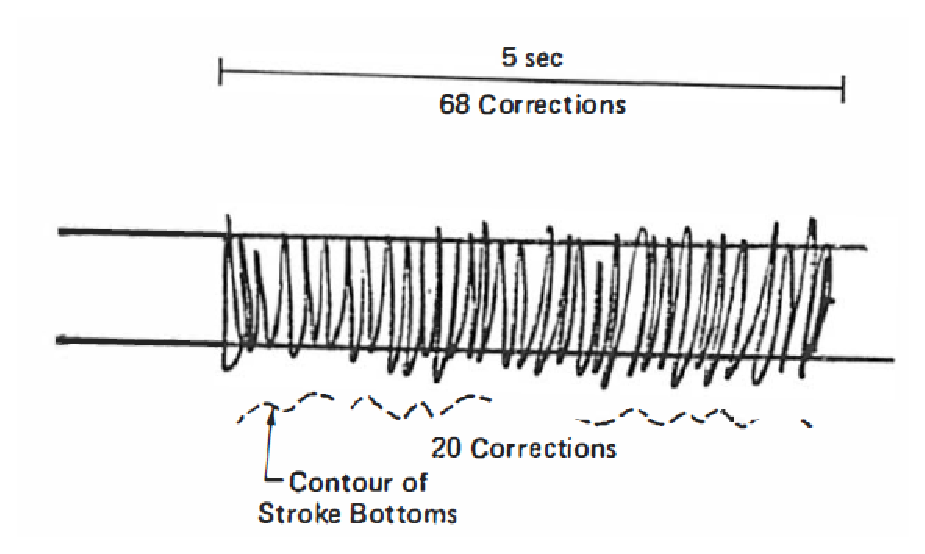
\includegraphics[width=0.5\hsize]{zigzag.eps}
 \end{center}
 \caption{ジグザグ運動の実験(図は[Wiley, 1978]のp.35より}
 \label{fig:zigzag}
\end{figure*}

一方、指の場合はキーボードを使った研究があり、
「同じキーを連続して打つ」という調査では、平均180[ms]/打(一回の運動あたり90[ms]; 押し上げと押し下げ)だそうです[Wiley, 1978]。
これは秒間打鍵に換算すると約5.6打/秒となります(あくまで同じキー連打の場合です)。

これを整理すると、表\ref{tbl:renzoku}のようになります。

\begin{table*}
\begin{center}
\caption{連続運動における所要時間}
\begin{tabular}{ccc}
\hline
鉛筆のジグザグ & 70[ms] (30~100[ms]) & 14回/秒 \\
腕・足・舌の繰り返し & 100[ms] & 10回/秒 \\
キーボード 同一キー連続 & 180[ms] & 5.6打/秒 \\
\hline
\end{tabular}
\label{tbl:renzoku}
\end{center}
\end{table*}

\subsubsection*{フィッツの法則}

以上のような知見を利用してモデルを立てることができます。
いま、距離$D$の場所に幅$S$(今は一次元の運動のみを考えます。
つまり、縦方向には無限に伸びているものとします)の物体があるとします。
この物体に腕・指を動かして触れる、というタスクを考えます(図\ref{fig:fitts})。

「目標物に対して腕・指を動かして触れる」という動作は一動作に見えますが、実はいくつもの離散的な運動の連鎖からなっています。
つまり、対象物との距離を計りながら少しずつ何度も何度もフィードバックさせ、減速や方向調整などをしています。

\begin{figure*}[htbp]
 \begin{center}
  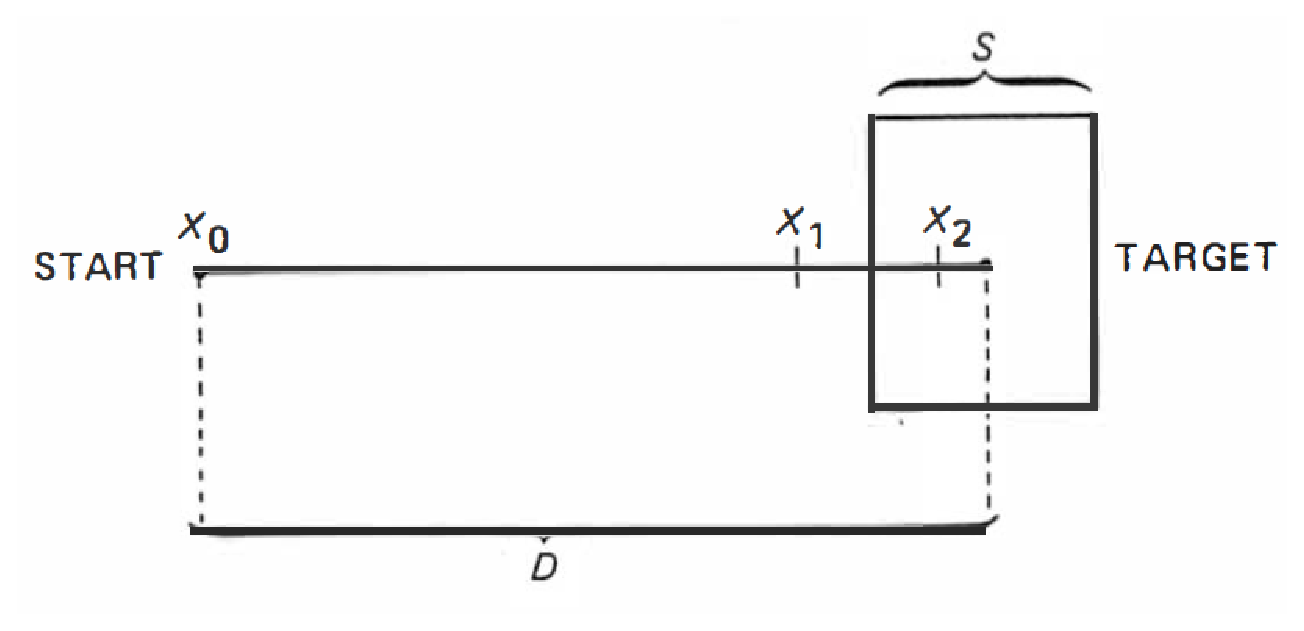
\includegraphics[width=0.5\hsize]{fitts.eps}
 \end{center}
 \caption{フィッツの実験}
 \label{fig:fitts}
\end{figure*}

ここからは専門的になるので導出はコラムに任せるとして、このタスクと所要時間$T$[ms]の間に、次のような法則が得られます:
\[
  T = I_M \log_2 \left(\frac{D}{S} + 0.5\right)
\]
ここで、$I_M$は100 [ms/bit]です\footnote{$\log$の中は無次元なので、一見無次元に見えますが、$\log$は底、つまり$\log_{e}$なのか$\log_{10}$なのかを区別するために、特別に単位をつけます。2を底とする場合は、bitをつけます。ちなみに前者$e$は\ruby{nat}{ナット}、$10$は\ruby{dit}{ディット}と言います。}%
(70~120)。

直感的には、こんな感じの説明になります。すごく遠いところにある(⇔$D$がとても大きい)と$T$は大きくなります。
一方、対象物がすごく大きい(⇔$S$がとても大きい)と、当然触れやすいので$T$は小さくなる、つまり速く押せます
(表\ref{tbl:fitts2})。

\begin{table}[htbp]
 \begin{center}
 \caption{フィッツの法則}
 \begin{tabular}{ccccc}
 \hline
  & {\bf\LARGE 近い} & $\cdots$ & {\bf\small 遠い} \\
  & \multicolumn{3}{c}{短時間 $\Longrightarrow$ 長時間} \\
  & {\bf\LARGE でかい} & $\cdots$ & {\bf\small 小さい} \\
 \hline
  \end{tabular}
  \label{tbl:fitts2}
\end{center}
\end{table}

%\begin{itembox}{{\bf コラム フィッツの法則の導出}}
\subsubsection{(発展:フィッツの法則の導出)}

\hspace{1zw}
「対象物との距離を計りながら動かす」離散的な動作を1サイクルと定義します。このとき、1サイクルごとに
\[
  T_{cycle} = T_p + T_C + T_M \simeq 240 {\mathrm ms}
\]
の時間がかかります。$T_p, T_C, T_M$は前に定義した値です。
$n$サイクルで対象物に到達するとすると、合計時間$T$は
\[
  T = n \cdot T_{cycle} = n ( T_P + T_C + T_M )
\]
となります。

ここで、$i$サイクル目での対象物への距離を$X_i$とします。$X_0 = D$です。1サイクルごとに制御する正確さは変わらないと仮定すると、
ある数$\epsilon < 1$を用いて$X_i = \epsilon X_{i-1}$と表すことができます({\bf 差}ではなく{\bf 比}を使うのがポイントです)。

すると、到達時の対象物への距離$X_n$(この時点でほとんどゼロに近くなっている)は
\[
X_n = \epsilon^n D
\]
と表せます。これが幅$S$に収まっていれば(=接触していれば)よいのですが、「行き過ぎ($+S/2$)」と「行き足りない($-S/2$)」があるので$1/2$します。つまり、
\[
  \epsilon^n D \le \frac{S}{2}
\]
これをnについて解くと、
\[
  n = -\log_2 (2D/S) / log_2 \epsilon
\]
この$n$を$T$の式に代入することによって、
\[
  T = I_M \log_2 (2D/S) \quad \mathrm{[ms]}
\]
を得ます。ただし、$I_M = -(T_P + T_C + T_M) / \log_2 \epsilon$です。

定数$\epsilon$はだいたい0.07とされています([Keele,1968][Vince,1948])。よって$I_M$は、
\begin{eqnarray*}
I_M &=& -240 / \log_2 (0.07) \\
    &=& 63 \quad \mathrm{[ms/bit]}
\end{eqnarray*}
となります。
\begin{flushright}
■
\end{flushright}
%\end{minipage}
%\end{itembox}

\subsubsection*{練習の効果 --- べき乗則}

さて、ここまでモデルを立てて計算してきたわけですが、人間はなにごとにも上達します。つまり、練習を重ねることによって、キーボードも速く打つことができます。

[Snoddy,1926]は、「ものを知覚してある運動をする時間」と練習量の間に次の関係を見出しました(Power Law of Practice)。
いわゆる{\bf 「べき乗則」(Power Law)}として知られている法則です。
\[
  n回目の試行における時間 T_n = T_1n^{-\alpha}
\]
ただし、$\alpha$はある定数です。

わかりやすくするために、$\alpha=1$としてみましょう。つまり、$T_n = T_1/n$です。この場合、2回目の試行で最初の試行の半分、3回目で三分の一、4回目で四分の一となります。グラフに表すと反比例のグラフになります。{\bf 最初のほうでぐっとタイムが縮まり、後のほうではタイムの縮まりは伸び悩んでいる}ことがわかりますね。

それをわかりやすく図示したのが、図\ref{fig:powerlaw}で、$y=1/\sqrt{x}\ (=1/x^{0.5}),\  y=1/x,\  y=1/x^2$のグラフです。上の式でいうと、それぞれ$\alpha = \frac{1}{2}$(実線)、$\alpha = 1$(破線), $\alpha = 2$(点線)の場合です。
$\alpha$が小さい(=実線になっていく)と、なかなかタイムが縮まりにくい(=縦軸が下がりにくい=タイムが縮まりにくい=上達しにくい)ことがわかりますね。

\begin{figure*}[htbp]
 \begin{center}
  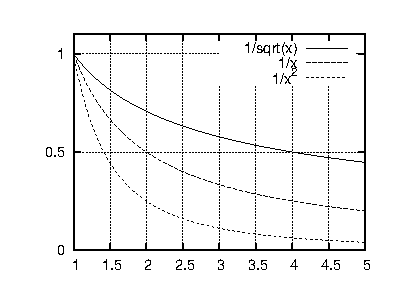
\includegraphics[width=0.7\hsize]{graph.eps}
 \end{center}
 \caption{べき乗則の例($y=1/\sqrt{x}$、$y=1/x$、$y=1/x^2$のグラフ)}
 \label{fig:powerlaw}
\end{figure*}

次に挙げる実験では、$\alpha = 0.38$という値が得られています。
(上で挙げた$1/\sqrt{x}$よりもさらに上達しにくい!)

詳しく説明しましょう。
図\ref{fig:powerlaw2}は[Klemmer,1962]による実験のグラフです。
Klemmerは、被験者に10個のボタン($2^{10} =1024$通り)のパターンを練習させました。

\begin{figure*}[htbp]
 \begin{center}
  \includegraphics[width=0.85\hsize]{powerlaw2.eps}
 \end{center}
 \caption{キー入力における べき乗則の実験(図は[Wiley, 1978]のp.59より}
 \label{fig:powerlaw2}
\end{figure*}

図\ref{fig:powerlaw2}を詳しく見てみましょう。両対数グラフになっているのでわかりにくいですが、たとえば{\bf 1000msから900msまで100ms縮めるのに1000回練習している}ことが、左から三番目と四番目の点からわかります。黒点はだいたい1000回ごとの練習を表しています。
また、$x$軸の10,000の右側、10000回目から20000回目の間に、点が密集しているのが見えますね。これは、{\bf 600msから500msまで100ms縮めるのに10000回もかかった}ということを表しています。1000ms→900msと比べて{\bf 10倍も練習量が必要}というのがわかります。

このように、ある$n$(ここでは練習回数)に対して、対応する関数$T(n)$(ここではタイム$T$)が$1/n$に比例することを、{\bf べき乗則}と言います。\footnote{余談ですが、自然界にはこのようにべき乗則が多く見られます。たとえば、ある文章中の単語を頻度順(多い順)に並べたときに、第$n$位の単語の文章中に占める割合は$1/n$にほぼ比例します({\bf Zipf(ジフ)の法則})。実際、theは文書中の7\%を占め、次にofがその半分の3.5\%を占めます。}

\subsubsection*{タイピング速度の理論と実際}

ここまで出てきた知識で、タイピング速度の理論値を計算してみましょう。

ものすごくざっくりと計算します。「鉛筆をひたすら速く上下させてジグザグ状に書く」という動作で測定した計測値$T_M = 30 \sim 100$[ms]を用います。キーを押すのには「押し下げ+押し上げ」の二動作がありますから、$2\times T_M$となります。
しかし、左右交互に押し下げ/押し上げを繰り返すので、結局のところ理論値は$T_M$となり、%
{\bf 秒間33打鍵~10打鍵(平均14打鍵/秒)}となります。実際には知覚による判断も入ってきますので、上限の33打鍵は不可能でしょう。

実際のところどのくらいまで速くなるのでしょうか?

表\ref{tbl:speed}に、タイプライタでの一ストロークあたりの時間を挙げます\footnote{おまけで他にも載せました。表の値は[Wiley, 1978]によります。}。文献による{\bf タイピングチャンピオンは60[ms/打]で、これは16.7[打/秒]に相当します}。タイプウェル国語Rや英単語(400打鍵)だと{\bf 24秒}で打ちきることができる試算になります。

\begin{table*}[htbp]
 \begin{center}
     \caption{タイプライタにおける打鍵速度}
 \begin{tabular}{lcc}
\hline
タイプライタ & [ms/打] & 秒間打鍵数[打/秒] \\
\hline
Best case(チャンピオン) & 60 & 16.7 \\
テキストタイピング & 158~231 & 4.3~6.3 \\
テキストタイピング(ランダム単語列) & 200~273 & 3.7~5 \\
テキストタイピング(ランダム文字列) & 462~500 & 2~2.2 \\
アルファベット手書き & 545~932(ms/字)  & 1.1~1.8 \\
\hline
 \end{tabular}
 \label{tbl:speed}
 \end{center}
\end{table*}

\subsubsection{各キーごとの実測}

キーボード入力の速さを、もう少し詳しく見た研究があります。図\ref{fig:kinkead1}はQWERTYキーボードにおける各キーの、
\begin{itemize}
 \item 同手打鍵
 \item 異手打鍵
 \item 同指打鍵
 \item 同キー連続
\end{itemize}
の四種類それぞれの条件下で打ったときにかかる時間を示しています[Kinkead,1975]。

例として一つ見てみましょう。図\ref{fig:kinkead_k}にKのキーを載せます。
左上の数値162は、同じ右手でキーを打ったとき、たとえば\key{O}\key{K}を打ったときに\key{K}を打つのにかかる時間を表しています。
同様に、右上の数値133は、左手で前のキーを打ったとき、例えば\key{C}\key{K}を打ったときに\key{K}を打つのにかかる時間を表しています
({\bf 同手打鍵よりも交互打鍵のほうが速い}、ということも見てとれますね)。

\begin{figure*}[tbp]
 \begin{center}
  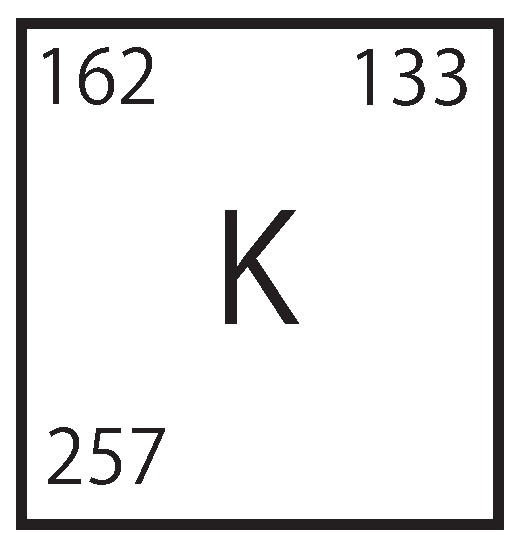
\includegraphics[width=0.15\hsize]{kinkead2.eps}
 \end{center}
 \caption{Kinkeadによるキー入力間の打鍵時間、Kの例}
 \label{fig:kinkead_k}
\end{figure*}

\begin{figure*}[htbp]
 \begin{center}
  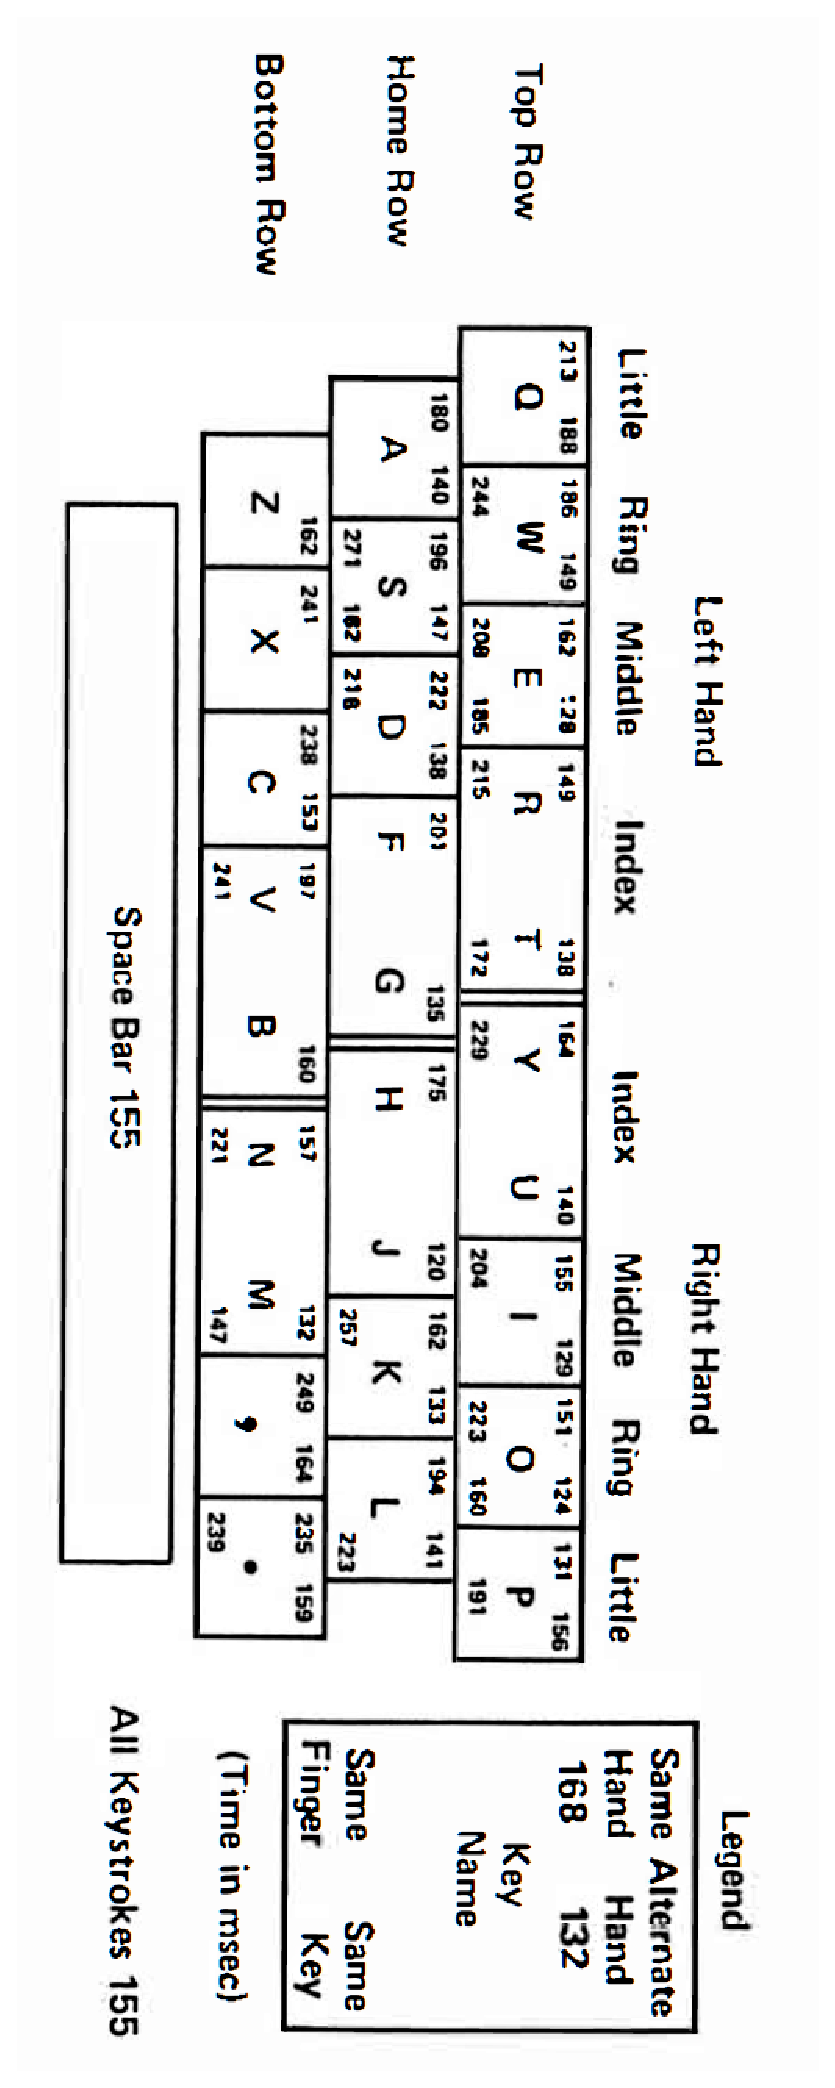
\includegraphics[height=0.9\vsize]{kinkead.eps}
 \end{center}
 \caption{Kinkeadによるキー入力間の打鍵時間(図は[Wiley, 1978]のp.62より}
 \label{fig:kinkead1}
\end{figure*}

Kinkead(1975) は図\ref{fig:kinkead1}の表の数値と、実際の英語の文字の出現頻度を用いて、タイピング時間を推計しました。
具体的には、2文字の連接(bigram)の頻度を用いて、
\[
  \mathrm{Typing rate} = \sum_i f_i t_i
\]
と計算しました。ただし、$f_i$はbigramの出現頻度、$t_i$はbigramに対応する図\ref{fig:kinkead1}の数値です。
この計算により、KinkeadはQWERTYのタイピング速度を162ms/打と推定しました。秒間打鍵に換算すると6.2打/秒となります。
Kinkeadは同じ計算をDvorakについても行い、QWERTYに比べて2.6\%しか速くなっていないということを示しました。

タイピング速度のシミュレーションを、このようなbigramの入力速度の総和で近似するという手法は、古典的ですが配列設計の最適化に役立つと言えましょう\footnote{ただし、Kinkeadのシミュレーション結果は「悪運指は良運指に悪影響を及ぼさない」という仮定をおいています。これは[Yamada, 1980a][Yamada, 1980b]の実験によって否定されています。今回は時間がなかったのでまた次回。}。

\section{配列解析編}

\subsection{はじめに}

この章では、世の中に存在する種々の配列のうちいくつかをピックアップして、それらについて定量的な分析を試みます。
具体的には「総打鍵数」「総打鍵数のうち、左・右の数・割合」「シフト数」「左手・右手の各指における使用数・比率」を見ます。
各段における使用比率も見ます。これは主として、ホームポジションから手が離れにくいかどうかを見る指標となります。
また、打ちやすさにおいて重要な因子となる、「連続して同じ指を使って打つ(同指異鍵; KIKIなど)」
「同じ手で段を二段以上飛び越えて打つ(同手跳躍; MIMIなど)」
「左手の縦の連続(左手縦連; WAZAWAZAなど)」も数えます。

以下にQWERTYローマ字入力を例にとって見てみましょう(表\ref{tbl:roma_example})。

まず一段目が、総打鍵数と、左手・右手での打鍵数とその比率です。シフト数はシフトを押した回数で、括弧内はクロスシフトです(NICOLA配列、中指シフト配列で効いてきます)。右側の「交互/左左/右右」は、二文字間での手の動きを示したものです。
二段目は各指の使用比率となっています。左から左小指、薬指、……、右小指となっています。
三段目は先行研究で議論されている「同じ指で違うキーを連続で打つ(同指異鍵)」「同じ手で段を二段以上飛び越えるキーを打つ(同手跳躍)」「左手で連続した縦のキーを打つ(左手縦連; \key{Z}\key{A}など)」の使用数、および各段ごとの使用比率となっています。


\begin{table*}[htbp]
 \caption{QWERTYローマ字の解析表}
 \begin{center}
 \begin{tabular}{cccc|ccc}
 \hline
総打鍵 & 総打鍵左 & 総打鍵右 & シフト数 & 交互 & 左左 & 右右 \\
37818164 & 16102479 & 21715685 & 7216(7216) & 17753448 & 7225755 & 12838961 \\
 & 42.6\% & 57.4\% & & 46.9\% & 19.1\% & 33.9\% \\
 \hline
 \end{tabular}

  \vspace{1zw} 

 \begin{tabular}{ccccccccccc}
 \hline
& 左小(A) & 左薬(S) & 左中(D) & 左人(FG) & 右人(HJ) & 右中(K) & 右薬(L) & 右小(;)\\
& 5180235 & 2405277 & 3120281 & 5396686 & 9531741 & 7001152 & 4679026 & 503766\\
左/右手中 & 32.2\% & 14.9\% & 19.4\% & 33.5\% & 43.9\% & 32.2\% & 21.5\% & 2.3\%\\
総打鍵中 & 13.7\% & 6.4\% & 8.3\% & 14.3\% & 25.2\% & 18.5\% & 12.4\% & 1.3\%\\
\hline
 \end{tabular}

  \vspace{1zw} 

 \begin{tabular}{ccc|cccc}
 \hline
 同指異鍵 & 同手跳躍 & 左手縦 & 最下段(ZX..) & ホーム(AS..) & 三段目(QW..) & 最上段(12..)\\
 2991366 & 5170649 & 3457 & 6024198 & 12333179 & 19265593 & 195194\\
  &  &  & 15.9\% & 32.6\% & 50.9\% & 0.5\%\\
%交互/左左/右右 中 & 交互/左左/右右 中 & 交互/左左/右右 中 &  &  &  & 総打鍵中 & 総打鍵中 & 総打鍵中 & 総打鍵中\\
\hline
 \end{tabular}
 \end{center}
 \label{tbl:roma_example}
\end{table*}

\subsection{QWERTYについて}

まず(個性的な)各配列に移る前に、研究が進んでいるQWERTYについて見てみることにします。その後、AZIK、かな配列と見ていきます。

\subsubsection*{QWERTYは「打ちやすい」か?}

みなさんがいちばん目にすることの多い配列、QWERTYはタイプライターの配列に始まります。1868年にはアルファベットをそのまま並べたものであったタイプライターの配列が、現在のQWERTY配列と同じものになったのは、1882年8月のことです(安岡孝一ら『キーボード配列QWERTYの謎』、NTT出版、2008年)。

QWERTYキーボードに対する批判は数多くあり、またそれらが他の配列を考案させる動機にもなっています。
(1983年当時の)過去50年間におけるQWERTY配列に対する批判をまとめると%
%\footnote{主としてDvorak博士とそのチームによる批判でした[Dvorak, 1943]。DvorakらのQWERTY配列批判は熾烈で、FIXME}%
[Noyes, 1983]、

\begin{enumerate}
\item 左手に過負荷である。キーの実行の57\%が、多くの人が利き腕でない左手により行われる%
    \footnote{これは英語の場合であることに注意してください。日本語の場合はこれと異なります。詳しくは後述のローマ字入力で。}
\item ある指にとって過負荷である\footnote{機械式のタイプライタでは、全ての指で同じ力を使って入力する必要がありました。そのため、小指や薬指など、力の弱い指に負担がかかることがあったようです。電動式になってから、この欠点はさほど問題ではなくなりました。}
\item 中段のキーの実行が少なすぎ(32\%)、上段のキーの実行が多すぎる(52\%)
\item よく使用される単語において、段の変更が多すぎる。しばしば下段、上段、下段となることがある。たとえば ``br, un, in''など。
\item 多くの一般用語が左手だけでタイプされる。たとえば ``was, were, extra, address''
\end{enumerate}

このうち3番目は補足が必要です。[Kinkead, 1975]によると、機械式のタイプライタでは中段のキーをおすのが最も速く、電気的なタイプライターでは上段のキー操作が最も速いと論じています(熟練したタイピストによる実験)。

\subsection{QWERTYローマ字入力}

さて、ここからは日本語タイピングについて議論していくことにします。
まずは、おそらく一番標準的な入力方式であるローマ字入力から。

QWERTYローマ字入力をコーパスを用いて評価すると表\ref{tbl:roma_example}のようになります。

日本語のタイピングにおいては、前述のNoyesの主張(左手偏重)に対して、
右手偏重の配列になっていることがうかがえます。
特に、右手人差し指の使用率が他の配列と比べ高くなっています。

この、右手偏重・右手人差し指偏重の結果については、次の点が原因として考えられます。
\begin{itemize}
\item 日本語は「子音+母音」で一文字となるがそのうち右手で打つ母音(\key{I}\key{O}\key{U})が母音中の約6割を占め、左手に比べてやや多いこと、
\item よく出る仮名の子音が、右手人差し指に集中していること、
\item[ ] \hspace{1zw}(頻度順に挙げると、「%
{\footnotesize い}%
\ruby{{\bf う}}{U}%
\ruby{{\bf ん}}{N}%
{\footnotesize し}%
\ruby{{\bf の}}{N}%
{\footnotesize かたと}%
\ruby{{\bf に}}{N}%
{\footnotesize て}%
\ruby{{\bf な}}{N}%
\ruby{{\bf は}}{H}」の太字)。
\end{itemize}

一方、左手の方は左小指の酷使がひどく、他の配列に比べ群を抜いています。「\ruby{笹}{ささ}沢(SASAZAWA)」などの「沢」が付く人名や、「わざわざ(WAZAWAZA)」の打ちにくさは、多くの人が経験していることと思います。

%\begin{table}[htbp]
% \begin{center}
%  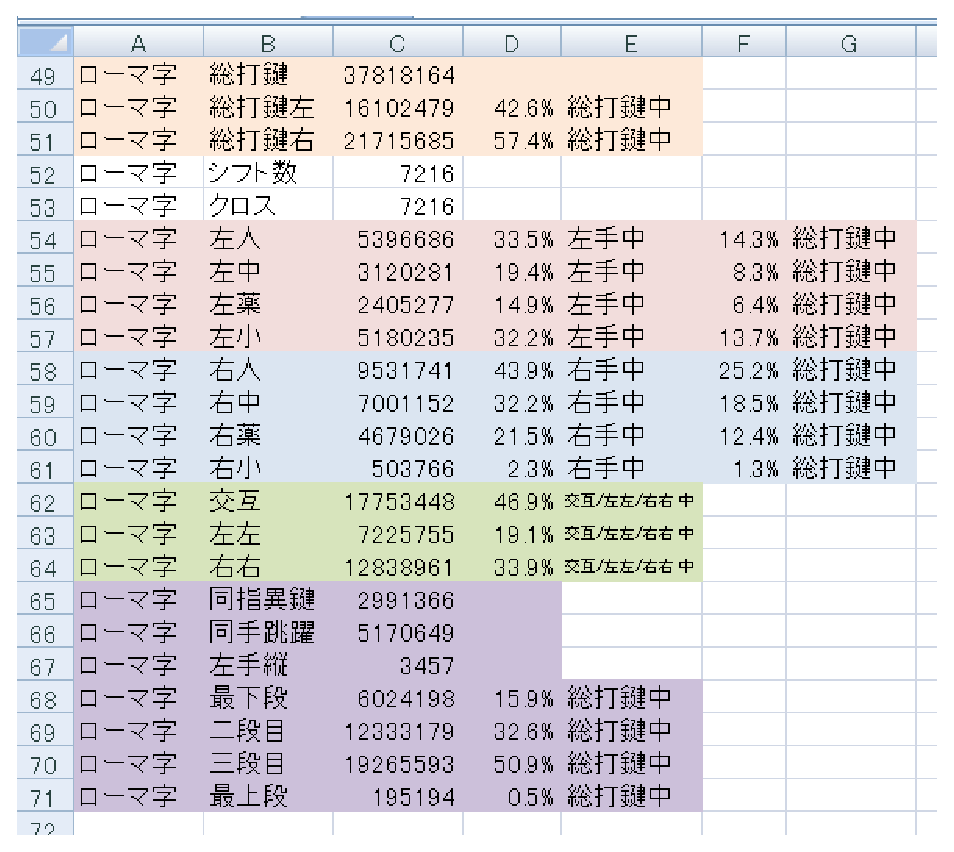
\includegraphics[width=0.85\hsize]{tbl-roma.eps}
% \end{center}
% \caption{QWERTYローマ字の解析表}
% \label{tbl:roma}
%\end{table}

\subsection{AZIK}

QWERTYによるローマ字入力を少し改良したのが、AZIKです。
AZIKでは、日本語の漢字の音の多くが「い」「ん」「う」
(「\ruby{会}{かい}」「\ruby{完}{かん}」「\ruby{項}{こう}」など)で終わることに着目しました。
より正確に言えば、ローマ字で書いて、-ai、-an、-ouなどの音で終わる文字が多い、ということです。
そこでAZIKでは、この``ai''、``an''に、一文字を割り当てることにしました。
たとえば``ai''は\key{Q}、``an''は\key{Z}です。日本語では、子音と母音が交互に連なることから「子音+子音」の組み合わせになったとき(たとえば``KZ'')のみ
\key{Z}をanと解釈すれば、「ざじずぜぞ」と競合することはありません%
\footnote{これは、ATOKやGoogle日本語入力のローマ字変換テーブルで容易に実装できます。}。%
日本語の漢字は全文章の約3割を占めますので、これらの漢字音の入力を省入力化すれば、全体的な打鍵数は少なくなります。

また、AZIKでは「っ」の文字を一文字(\key{;})で入力したり、頻出の「する」「こと」などを``sr''、``kt''で入力するなど、随所に省入力化が見られます。

その他特筆すべきこととして、きゃ行、ひゃ行、みゃ行などの\ruby{拗}{よう}音について、``KYU''などではなく``KGU''でも打てるようにしている点があります。これは省入力化ではなく、左右交互打鍵を狙った改良です。このような交互打鍵を目的とした拡張として、「だん」(DZ)を``DN''でも打てるようにしたものもあります。

さて、AZIKをコーパスを使って評価してみましょう。
%AZIKについては、作者が省入力化に段階を設けていますので、二種類の評価設定をとりました。具体的には、「AZIK総合解説書\footnote{{\tt http://hp.vector.co.jp/authors/VA002116/azik/azikinfo.htm}}」にある「その2(拡張キー)」のみのと、「その3」まで全て使用した場合の二通りです。
評価には、
\begin{itemize}
 \item \ruby{撥}{はつ}音拡張(-anなど, キー:ZNKJDL)(\key{Z}と\key{N}については、前節で述べた交互打鍵の優位性を\ruby{鑑}{かんが}みて、交互打鍵になるように各キーを選択しました)
 \item 二重母音拡張(-aiなど、キー:QHWP)
 \item 「し」「しょう」などshの音を\key{x}で入力 / 「ち」などchの音を\key{c}で入力
 \item 「ん」「っ」をそれぞれ\key{Q}, \key{;}で入力
 \item \ruby{拗}{よう}音を\key{Y}ではなく\key{G}で入力
 \item 「する」「こと」などをそれぞれ\key{S}\key{R}、\key{K}\key{T}などで入力
\end{itemize}
という設定を用いました。これは「AZIK総合解説書\footnote{\url{http://hp.vector.co.jp/authors/VA002116/azik/azikinfo.htm}}」にある、「その3」までの設定をほぼ踏襲しています。

%\begin{table}[htbp]
% \begin{center}
%  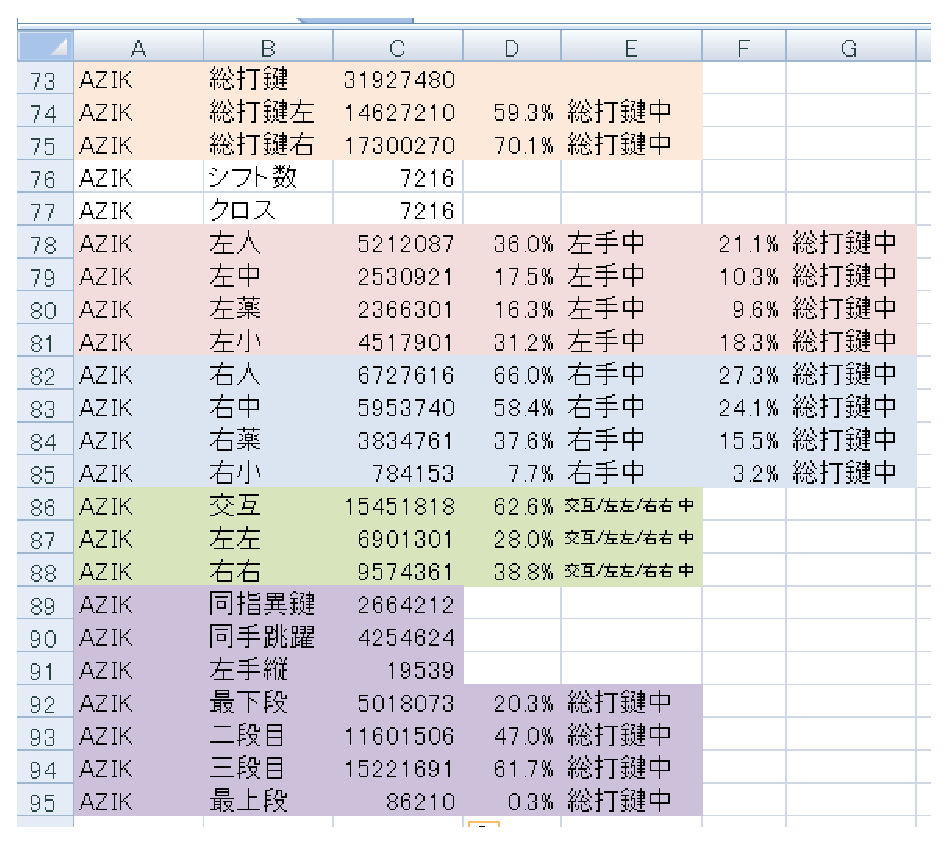
\includegraphics[width=0.85\hsize]{tbl-azik.eps}
% \end{center}
% \caption{AZIKの解析表}
% \label{tbl:azik}
%\end{table}

\begin{table*}[htbp]
 \caption{AZIKの解析表}
 \begin{center}
 \begin{tabular}{cccc|ccc}
 \hline
総打鍵 & 総打鍵左 & 総打鍵右 & シフト数(クロス) & 交互 & 左左 & 右右 \\
30200816 & 14072150 & 16128666 & 98014(9948) & 15211220 & 6466540 & 8523056 \\
 & 46.6\% & 53.4\% &  & 50.4\% & 21.4\% & 28.2\% \\
 \hline
 \end{tabular}

  \vspace{1zw} 

 \begin{tabular}{ccccccccccc}
 \hline
& 左小 & 左薬 & 左中 & 左人 & 右人 & 右中 & 右薬 & 右小 \\
& 3998593 & 2366304 & 2145980 & 5561273 & 6426213 & 5422220 & 3496080 & 784153 \\
左/右手中 & 28.4\% & 16.8\% & 15.2\% & 39.5\% & 39.8\% & 33.6\% & 21.7\% & 4.9\% \\
総打鍵中 & 13.2\% & 7.8\% & 7.1\% & 18.4\% & 21.3\% & 18.0\% & 11.6\% & 2.6\% \\
\hline
 \end{tabular}

  \vspace{1zw} 

 \begin{tabular}{ccc|cccc}
 \hline
 同指異鍵 & 同手跳躍 & 左手縦 & 最下段(ZX..) & ホーム(AS..) & 三段目(QW..) & 最上段(12..)\\
2030767 & 3797767 & 15170 & 5018292 & 11429889 & 13666425 & 86210 \\
 &  &  & 16.6\% & 37.8\% & 45.3\% & 0.3\% \\
%交互/左左/右右 中 & 交互/左左/右右 中 & 交互/左左/右右 中 &  &  &  & 総打鍵中 & 総打鍵中 & 総打鍵中 & 総打鍵中\\
\hline
 \end{tabular}
 \end{center}
 \label{tbl:azik}
\end{table*}

さてAZIKは、QWERTYローマ字(約3782万字)に比べ、約20\%打鍵数を削減できています。これは前述の二重母音などの省入力に加え、日本語で頻出の「する」「こと」を2ストロークで入力できるようにしたことも大きいのでしょう%
\footnote{ちなみに2000万字のコーパスでは、「する」は57752回、「こと」は88757回出ていました。}。

左手の子音のキーを多用することから、左手の使用率は若干高くなりました。
しかし、\key{Q}/\key{Z}を打つべき左手小指については、ローマ字の13.7\%に比べてAZIKが13.2\%と、ほとんど変わっていません。

AZIKの配置は覚えやすさのために、対応する母音のキーの近く(-ai/-anなら\key{A}の近くの\key{Q}と\key{Z})
という条件を設けていました。そのため、キーボード配列の打ちやすさという観点から言えばむしろ、
不利なものとなってしまう危険性を持っています。

実際、上で述べたような工夫を使わず、単純な\ruby{撥}{はつ}音拡張(ZKJDL)、二重母音拡張(QHWP)だけを使った
予備実験では、\key{A}と\key{E}が左手にあること、\key{Q}と\key{Z}が左手小指であることに引きづられて、
左手小指・薬指を酷使する配列になってしまっていました。

AZIKは、省入力化の方法をふんだんに用い、さらに交互打鍵まで考慮した結果として、
覚えやすさと効率を両方カバーした、バランスのとれた配列になった、と言えるでしょう%
\footnote{ただし、``sr''→する、以外の比較的頻度の低い二文字が覚えやすいかどうかは議論の余地があります。}。

%原理上、``ai''などのキーはどの子音のキーに置いてもよいため、これについては改良が望めます%
%\footnote{そのため、筆者(nooyosh)はいまYAZIK: Yet another AZIKという配列を考えているので、次回以降乞うご期待。}。

\subsection{JISかな}

みなさんご存じの「たていすかんなにらせ」――JISかな%
\footnote{次に説明する「新JIS配列」との比較で「旧JIS」と呼ばれることもあります。}%
は、当初カナタイプライタの配列から考案され、1972年にJISC 6233として制定されました。特徴としては、(ほぼ)すべてのキー使って仮名を配置しようとしたために、キーを四段すべて使っている点です。
後述する親指シフトや中指シフトなどのように、シフトキーを押す必要がないために直感的ではあるのですが、
\begin{itemize}
\item 上から二段目の使用頻度が高く、ホームポジションから指が離れやすい
\item 打鍵が左手に偏っている
\item 数字を打つときにカナキーを押す必要がある
\end{itemize}
など、いろいろと欠点があります。

詳しく見てみましょう(表\ref{tbl:jiskana})

\begin{table*}[htbp]
 \caption{JISかなの解析表}
 \begin{center}
 \begin{tabular}{cccc|ccc}
 \hline
総打鍵 & 総打鍵左 & 総打鍵右 & シフト数 & 交互 & 左左 & 右右 \\
24675899 & 14475950 & 10199949 & 2666111(2213255) & 11525084 & 8713408 & 4437407\\
 & 58.7\% & 41.3\% &  & 46.7\% & 35.3\% & 18.0\%\\
 \hline
 \end{tabular}

  \vspace{1zw} 

 \begin{tabular}{ccccccccccc}
 \hline
& 左小(A) & 左薬(S) & 左中(D) & 左人(FG) & 右人(HJ) & 右中(K) & 右薬(L) & 右小(;)\\
& 5609655 & 3528341 & 2956460 & 2381494 & 3483694 & 2418311 & 2048886 & 2249058\\
左/右手中 & 38.8\% & 24.4\% & 20.4\% & 16.5\% & 34.2\% & 23.7\% & 20.1\% & 22.0\%\\
総打鍵中 & 22.7\% & 14.3\% & 12.0\% & 9.7\% & 14.1\% & 9.8\% & 8.3\% & 9.1\%\\
\hline
 \end{tabular}

  \vspace{1zw} 

 \begin{tabular}{ccc|cccc}
 \hline
 同指異鍵 & 同手跳躍 & 左手縦 & 最下段(ZX..) & ホーム(AS..) & 三段目(QW..) & 最上段(12..)\\
4885493 & 3477500 & 487390 & 4477353 & 6071650 & 10022415 & 4104481\\
 &  &  & 18.1\% & 24.6\% & 40.6\% & 16.6\%\\
\hline
 \end{tabular}
 \end{center}
 \label{tbl:jiskana}
\end{table*}

%\begin{table}[htbp]
% \begin{center}
%  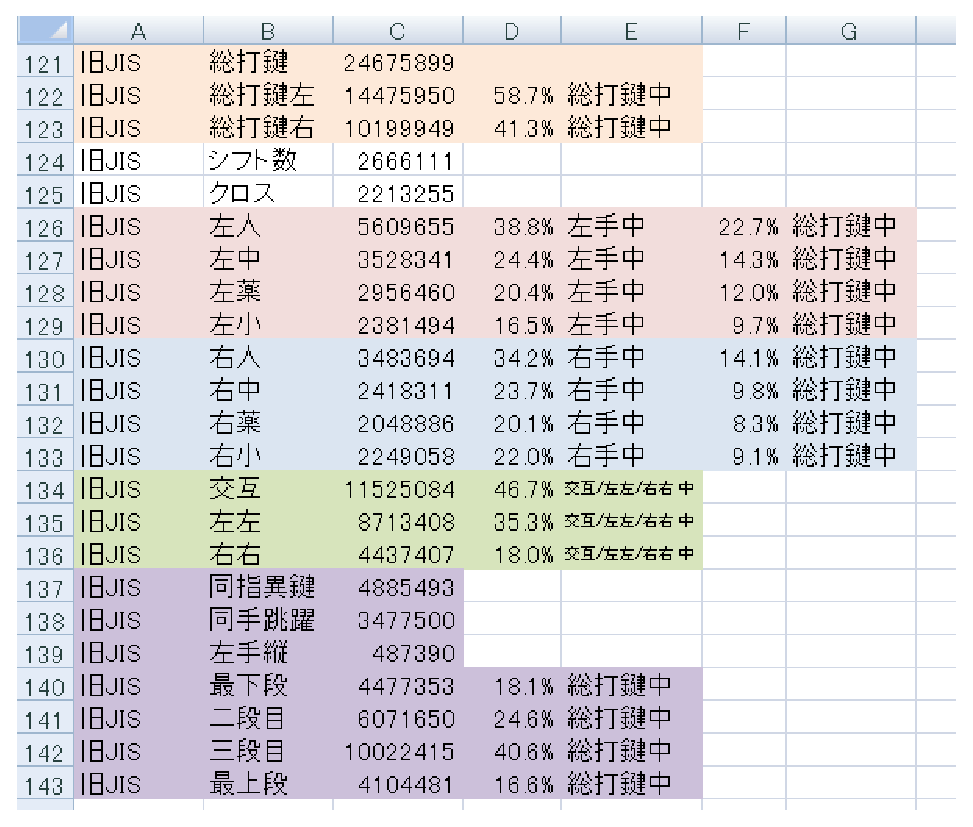
\includegraphics[width=0.85\hsize]{tbl-jiskana.eps}
% \end{center}
% \caption{旧JISの解析表}
% \label{tbl:jiskana}
%\end{table}

総打鍵中約6割が左手になります。そのうち、左人差し指が総打鍵の約23\%を占めるなど、著しい偏りが見られます(「う」「か」などが左人差し指の高頻度文字)。
bigram、つまり二文字列の連なりを見ても、左手→左手の組み合わせが4割弱と、左手の酷使が見て取れます(「てい」「った」など)。
また、上から二段目(QWE...)が総打鍵の約4割を占めるなど、ホームポジションから指が離れやすい点も確認できます。

\subsection{新JIS系・中指シフト系カナ配列}
\subsubsection*{新JIS}

JISかなの欠点を解消するため、1986年に新しい仮名配列がJISで決定されました。
これは、「頻度の比較的低いキーはシフトで入力させ、指がホームポジションからなるべく離れないようにする」という設計思想に基づいて考案された配列です。
一般に新JISと呼ばれます。
しかし、JISかなが廃止されずに併存したことから、新JISは全く普及せず、「使用実態がない」として1999年に廃止されてしまいました。

新JISの設計では、キーボード最上段(数字キーのある段)の入力スピードが、他の段に比べて遅いことに注目しました。
ホームポジションから遠いキーの入力が遅いことは、前述のフィッツの法則(遠くにある小さいキーほど入力速度が遅い)からもわかります。
そこで、新JISでは仮名をすべて三段に収めようとしました。三段では足りないので、出現頻度の低い文字についてはシフトキーを用いて入力するようにしました(「裏に配置」)。

次に、どう仮名を配置するかです。まず考慮されるべきは、出現頻度です。これに関しては、高校教科書の文章の「1文字の出現頻度」(unigramの頻度)、「2文字の連接の出現頻度」(bigramの頻度)が用いられました。

具体的には、次の1.から4.のステップを経ます。

\begin{enumerate}
\item 「1文字の出現頻度」が高い順(「い」「う」「ん」……)に仮名を並べ、半数を「シフトしないで入力されるキー」(「表」; アンシフト)に設定します。
例えば、「い」は日本語の文章で一番多く出現するため、当然表に出てきます。
\item これらを、交互打鍵率が最大になるように左右に分けました。「交互」の計算には、上であげたbigramを用います。これも上であげた「2文字の連接」(bigram)を使います。
    「てい」はとても多く(bigram全体の約0.7\%)見られるので、\key{て}と\key{い}のキーは(なるべく)左右に分離して配置した方がよいことになります。
\item 左右グループそれぞれについて、指の段越えが少なくなるような組み合わせを探します。
\item さらに、左右グループそれぞれについて、同じ指が連続して打つ(同指異鍵)回数が少なくなるような組み合わせを探します。
\end{enumerate}

シフトされる仮名の集合については、シフトキーを1ストロークと見なして、交互打鍵の頻度が最大になるように左右グループにわけ、さらにホームポジションの段に頻度の高い仮名を配列するようにしました。

これもコーパスを使って見てみましょう(表\ref{tbl:newjis})

\begin{table*}[htbp]
 \caption{新JISの解析表}
 \begin{center}
 \begin{tabular}{cccc|ccc}
 \hline
総打鍵 & 総打鍵左 & 総打鍵右 & シフト数 & 交互 & 左左 & 右右 \\
24706219 & 11010567 & 13695652 & 4031578\\
 & 44.6\% & 55.4\% & \\
 \hline
 \end{tabular}

  \vspace{1zw} 

 \begin{tabular}{ccccccccccc}
 \hline
& 左小(A) & 左薬(S) & 左中(D) & 左人(FG) & 右人(HJ) & 右中(K) & 右薬(L) & 右小(;)\\
& 4738263 & 2648262 & 2256137 & 1367905 & 5212719 & 3530762 & 3702200 & 1249971\\
左/右手中 & 43.0\% & 24.1\% & 20.5\% & 12.4\% & 38.1\% & 25.8\% & 27.0\% & 9.1\%\\
総打鍵中 & 19.2\% & 10.7\% & 9.1\% & 5.5\% & 21.1\% & 14.3\% & 15.0\% & 5.1\%\\
\hline
 \end{tabular}

  \vspace{1zw} 

 \begin{tabular}{ccc|cccc}
 \hline
 同指異鍵 & 同手跳躍 & 左手縦 & 最下段(ZX..) & ホーム(AS..) & 三段目(QW..) & 最上段(12..)\\
2495822 & 830701 & 38977 & 4876067 & 13254518 & 6496686 & 78948\\
 &  &  & 19.7\% & 53.6\% & 26.3\% & 0.3\%\\
\hline
 \end{tabular}
 \end{center}
 \label{tbl:newjis}
\end{table*}



%\begin{table}[htbp]
% \begin{center}
%  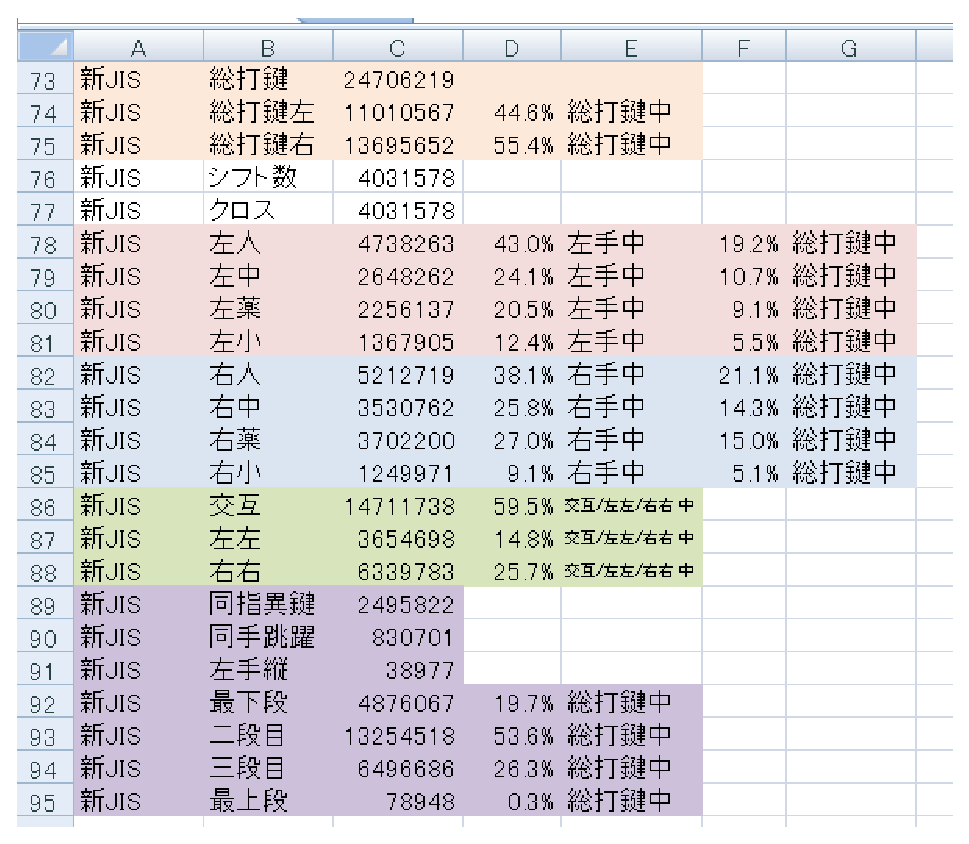
\includegraphics[width=0.85\hsize]{tbl-newjis.eps}
% \end{center}
% \caption{新JISの解析表}
% \label{tbl:newjis}
%\end{table}

右手と左手の\ruby{乖離}{かいり}が若干改善されました。また、交互打鍵が全体の約6割と、JISかなの約46\%と比べて大幅に改善されたことがわかります。
また、JISかなで38\%あった「左左」が15\%と、劇的に少なくなっています。上から三段目(ホームポジション)での打鍵が約54\%と、あまり指がホームポジションから離れないということも示唆されます。

\subsubsection*{花配列}

花配列は、冨樫雅文氏によって考案された、中指シフトと呼ばれる新しい配列です(図\ref{fig:hana}%
\footnote{図は「花のくに」\url{http://homepage3.nifty.com/togasi/hana_no_kuni/index.html} より。}%
)。新JIS配列では、仮名をホームポジション近くに収めるために、
シフトキーを用いていました。シフトキーはキーボードの右端と左端に置かれていますので、このままでは小指を酷使してしまいます。

そこで、冨樫氏は新しいシフト方式を考案しました。シフトキーを中指、QWERTYでいうDとKの位置に置き、しかもシフトを押すといったんロックされ、次の入力とともに解除される方式をとりました。
冨樫氏のこの方式は、中指シフト配列という新たな配列の分野を切り開いた、画期的な配列であると言えるでしょう。

さて、花配列では、「最もよい配列」を次のように定義しました。

\begin{itemize}
\item 1文字あたりの平均入力速度が最も速い
\item 各指にかかる負荷があらかじめ指定したものに最も近い
\end{itemize}

これらを定量的に明らかにするために、
\begin{itemize}
\item 仮名文字の使用頻度
\item 打鍵速度(打鍵間の所要時間)
\item 指の使用頻度分布
\end{itemize}
が使われました。
実際の配列設計では、まずランダムに配列を決定し、少しずつ(上の基準をみたすように)変化させていき、変化しなくなるまで10000回行いました。
これは、いわゆる焼きなまし法(Simulated Annealing)を行なっていたと考えられます。

ではコーパスを使ってみてみましょう\footnote{%
なお、シフトについては全てクロスシフトになるように(有利に)評価しました。
これについては評価がわかれる(アルペジオなど)ところですが、交互打鍵が最速という先行研究にしたがい、
クロスシフトを採用しました。以下の月配列などについても同様の設定です。}(表\ref{tbl:hana})。
%\begin{table}[htbp]
% \begin{center}
%  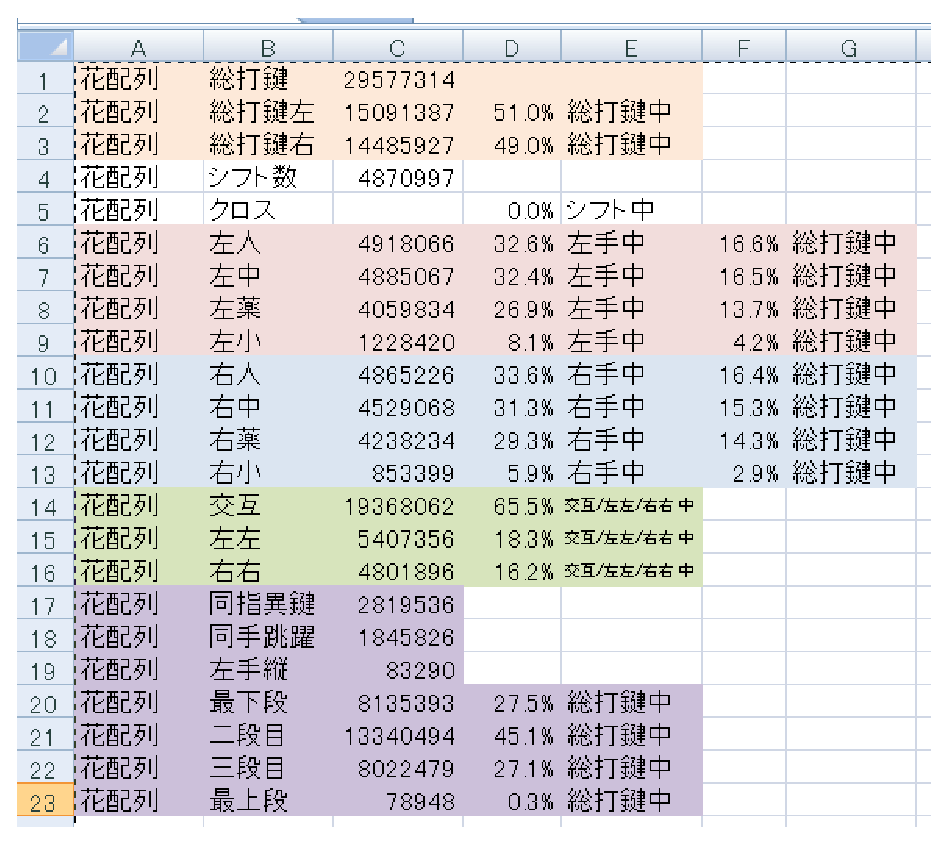
\includegraphics[width=0.85\hsize]{tbl-hana.eps}
% \end{center}
% \caption{花配列の解析表}
% \label{tbl:hana}
%\end{table}

\begin{table*}[htbp]
 \caption{花配列の解析表}
 \begin{center}
 \begin{tabular}{cccc|ccc}
 \hline
総打鍵 & 総打鍵左 & 総打鍵右 & シフト数 & 交互 & 左左 & 右右 \\
29577314 & 15091387 & 14485927 & 4870997 & 19368062 & 5407356 & 4801896\\
 & 51.0\% & 49.0\% &  & 189.7\% & 53.0\% & 47.0\%\\
 \hline
 \end{tabular}

  \vspace{1zw} 

 \begin{tabular}{ccccccccccc}
 \hline
& 左小(A) & 左薬(S) & 左中(D) & 左人(FG) & 右人(HJ) & 右中(K) & 右薬(L) & 右小(;)\\
& 4918066 & 4885067 & 4059834 & 1228420 & 4865226 & 4529068 & 4238234 & 853399\\
左/右手中 & 32.6\% & 32.4\% & 26.9\% & 8.1\% & 33.6\% & 31.3\% & 29.3\% & 5.9\%\\
総打鍵中 & 16.6\% & 16.5\% & 13.7\% & 4.2\% & 16.4\% & 15.3\% & 14.3\% & 2.9\%\\
\hline
 \end{tabular}

  \vspace{1zw} 

 \begin{tabular}{ccc|cccc}
 \hline
 同指異鍵 & 同手跳躍 & 左手縦 & 最下段(ZX..) & ホーム(AS..) & 三段目(QW..) & 最上段(12..)\\
2819536 & 1845826 & 83290 & 8135393 & 13340494 & 8022479 & 78948\\
 &  &  & 27.5\% & 45.1\% & 27.1\% & 0.3\%\\
\hline
 \end{tabular}
 \end{center}
 \label{tbl:hana}
\end{table*}

\begin{figure*}[htbp]
 \begin{center}
  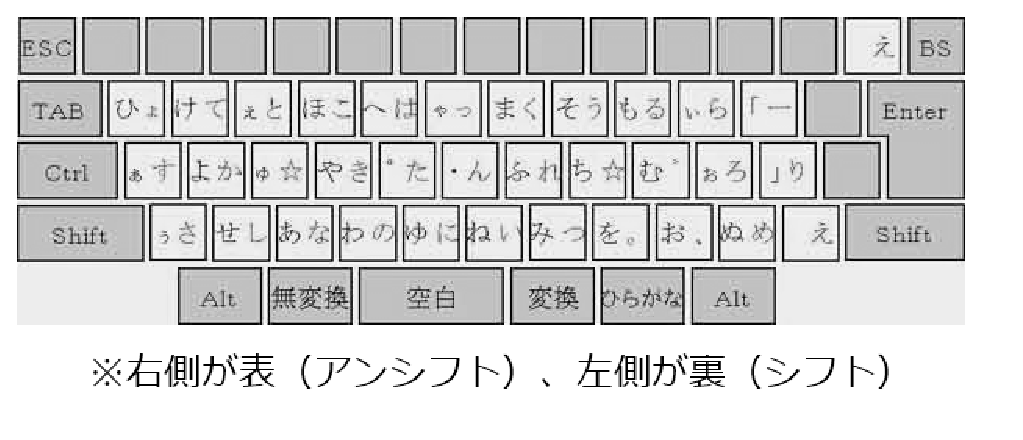
\includegraphics[width=0.8\hsize]{hana.eps}
 \end{center}
 \caption{花配列}
 \label{fig:hana}
\end{figure*}


新JISと同様、交互打鍵が約6割と多くなっています。
一方、新JISに比べ(18\%)、最下段が31\%となっており、これはJISかなの16\%と比較しても多く使われています。
これについて、冨樫氏は「手首を浮かせて打つと楽に打てる」と主張しています。

ただし、同手跳躍、同指異鍵などは、今回使用したコーパスでは新JISのほうが少なくなっていました。これは使用している文章の分野(ドメイン)の問題も大きくあると考えられます。

\subsubsection*{月配列}

2chの新JISスレッドでできたカナ系配列で、新JISに対して、前述の花配列のような中指シフトを付け加える、というアイディアのもと生まれました。
2chのスレッドにいるさまざまな人たちによって改良が重ねられ、多くの版(配列)ができました。現在では2-263(図\ref{fig:tsuki}%
\footnote{図は\url{http://jisx6004.client.jp/tsuki.html}より。}%
)と呼ばれているものが一般的です。

\begin{figure*}[htbp]
 \begin{center}
  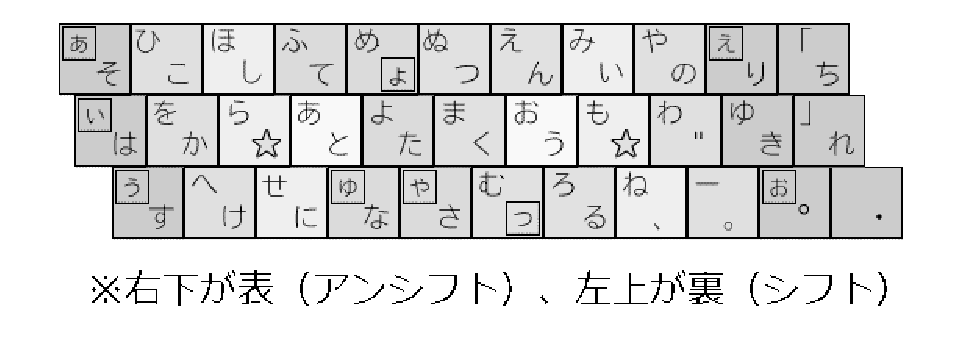
\includegraphics[width=0.8\hsize]{tsuki.eps}
 \end{center}
 \caption{月配列}
 \label{fig:tsuki}
\end{figure*}

コーパスを使ったこの配列の解析は表\ref{tbl:tsuki}のようになります。

\begin{table*}[htbp]
 \caption{月配列の解析表}
 \begin{center}
 \begin{tabular}{cccc|ccc}
 \hline
総打鍵 & 総打鍵左 & 総打鍵右 & シフト数 & 交互 & 左左 & 右右 \\
29526169 & 14294112 & 15232057 & 4819852 & 19309588 & 4639318 & 5577263\\
 & 48.4\% & 51.6\% &  & 65.4\% & 15.7\% & 18.9\%\\
 \hline
 \end{tabular}

  \vspace{1zw} 

 \begin{tabular}{ccccccccccc}
 \hline
& 左小(A) & 左薬(S) & 左中(D) & 左人(FG) & 右人(HJ) & 右中(K) & 右薬(L) & 右小(;)\\
& 5143242 & 5125313 & 2677655 & 1347902 & 4910816 & 5151515 & 4143342 & 1026384\\
左/右手中 & 36.0\% & 35.9\% & 18.7\% & 9.4\% & 32.2\% & 33.8\% & 27.2\% & 6.7\%\\
総打鍵中 & 32.2\% & 14.9\% & 19.4\% & 33.5\% & 43.9\% & 32.2\% & 21.5\% & 2.3\%\\
\hline
 \end{tabular}

  \vspace{1zw} 

 \begin{tabular}{ccc|cccc}
 \hline
 同指異鍵 & 同手跳躍 & 左手縦 & 最下段(ZX..) & ホーム(AS..) & 三段目(QW..) & 最上段(12..)\\
2322072 & 996617 & 50003 & 5138841 & 15676342 & 8632038 & 78948\\
 &  &  & 17.4\% & 53.1\% & 29.2\% & 0.3\%\\
\hline
 \end{tabular}
 \end{center}
 \label{tbl:tsuki}
\end{table*}

%\begin{table}[htbp]
% \begin{center}
%  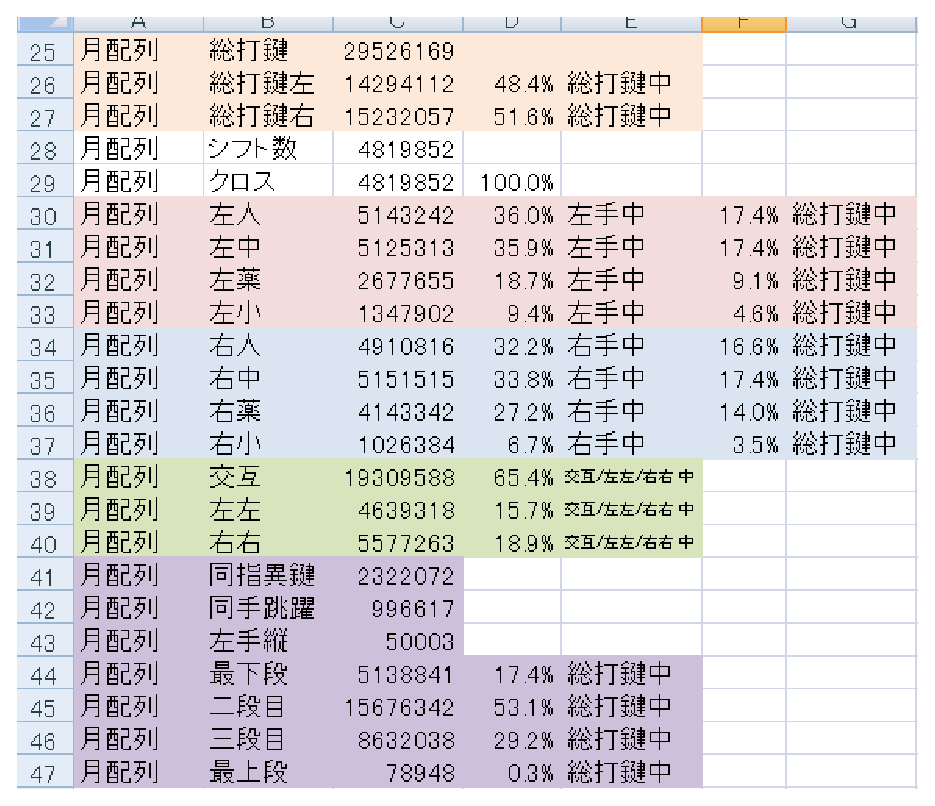
\includegraphics[width=0.85\hsize]{tbl-tsuki.eps}
% \end{center}
% \caption{月配列の解析表}
% \label{tbl:tsuki}
%\end{table}

新JISの持っていた6割という交互打鍵率をこの配列も保っています。新JISに比べ、左左/右右がバランスよく含まれており、両手をより均等に使った配列と言えるでしょう。

\subsection{親指シフト系}
\subsubsection*{NICOLA}

OASYS配列、またはNICOLA配列は「親指シフト配列」と呼ばれ、
キーボードのスペースキーにあたるところに、図\ref{fig:nicola}のような二つの「親指シフトキー」をおいてあるのが特徴です。

図\ref{fig:nicola}のキーには三つ仮名が書いてありますね。
下にある文字はそのまま打ち、上にある文字は「その文字と同じ手でシフトを押しながら」(同手シフト)打ちます。
濁音については、「清音のキーと反対側の手でシフトを押しながら」(クロスシフト)打ちます。
この仕様のため、親指シフトでは、清音(濁音が付く文字)はすべて単独で打てる文字となっています。

\begin{figure*}[htbp]
 \begin{center}
  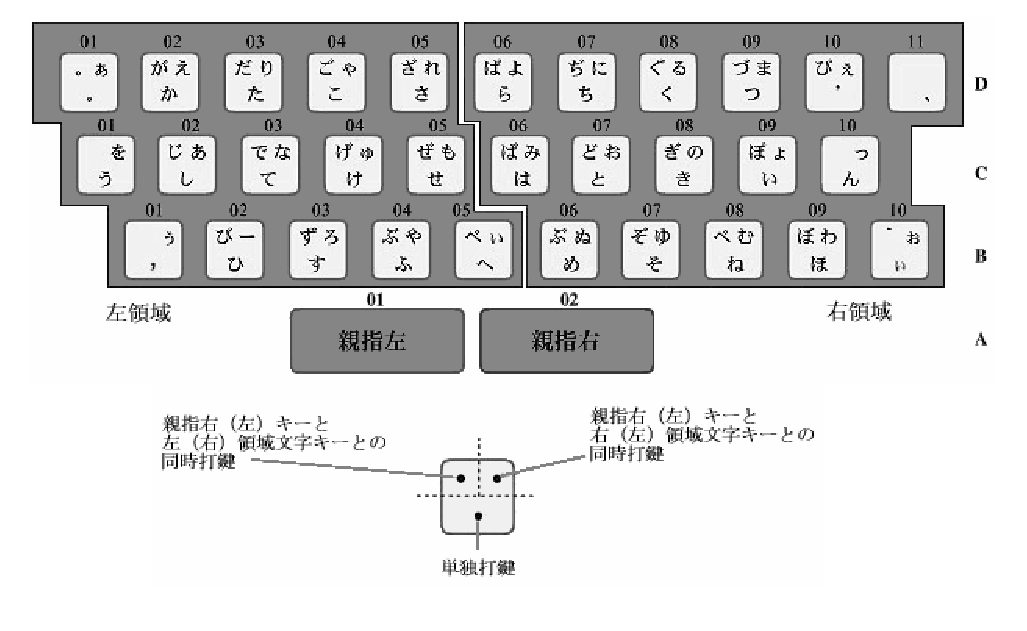
\includegraphics[width=0.8\hsize]{nicola.eps}
 \end{center}
 \caption{NICOLA配列(図はNICOLA配列規格書より)}
 \label{fig:nicola}
\end{figure*}

親指シフト配列の起源は、1980年、富士通のOASYS100というワープロ専用機に始まります。
初代以降、一貫してOASYSは親指シフトを採用し、多くの支持者を生んできました。
日本語に適した入力方式の普及と標準化を目的として、1989年に発足した業界団体「日本語入力コンソーシアム」は、
富士通の親指シフトキーボードを改良し、「NICOLA配列」を提唱しました。

具体的な相違点としては、OASYSでは半濁音を「半濁音キー」を用いて押していたのに対し、
NICOLAでは親指で押せるようにしました。
また、最上段の記号や、バックスペース、改行キーなどの位置をNICOLAではJIS規格のキーボードに合わせています。

「キーボードを科学する」\footnote{\url{http://www.fmworld.net/oasysworld/cat/dgt01.html}}%
によると、
\begin{itemize}
\item 「人差し指がいちばん使いやすく、小指がいちばん使いにくい」
\item 「指の使いやすさは、中段(ホームポジション)、上段、下段の順」
\item 「同じ指、隣り合った指の使用は避ける」
\item 「同じ側の手ではなく、左右交互に使う方が打ちやすい」
\end{itemize}
また、(神田ら, 1979)によると
\begin{itemize}
\item 「文字の出現頻度および連接出現頻度」(unigramとbigram)を考慮
\end{itemize}
という設計思想に基づいてデザインされました。

神田らは(初代OASYSの親指シフト配列の)評価として、6人に一日0.5~1.5時間の練習を一ヶ月行わせました。その実験により、
\begin{itemize}
\item 文字キーは完全にタッチタイピングできる
\item 文字キーと親指シフトキーを同時に押すのは、キーを単独で打つのと同じ感覚で行える
\end{itemize}
ことがわかり、さらに打鍵速度として80~180字/分が得られたということです。

それではコーパスを使ってみてみましょう(表\ref{tbl:nicola})。ここでは多くの親指シフトエミュレータで採用されているNICOLA配列を評価することにします。

\begin{table*}[htbp]
 \caption{NICOLAの解析表}
 \begin{center}
 \begin{tabular}{cccc|ccc}
 \hline
総打鍵 & 総打鍵左 & 総打鍵右 & シフト数 & 交互 & 左左 & 右右 \\
 22009710 & 11180976 & 10828734 & 9331864(2892628) & 11729133 & 5316409 & 4964168\\
 & 50.8\% & 49.2\% &  & 53.3\% & 24.2\% & 22.6\%\\
 \hline
 \end{tabular}

  \vspace{1zw} 

 \begin{tabular}{ccccccccccc}
 \hline
& 左小(A) & 左薬(S) & 左中(D) & 左人(FG) & 右人(HJ) & 右中(K) & 右薬(L) & 右小(;)\\
& 2817456 & 3264915 & 3278771 & 1819834 & 3709821 & 2606899 & 2770957 & 1741057\\
左/右手中 & 25.2\% & 29.2\% & 29.3\% & 16.3\% & 34.3\% & 24.1\% & 25.6\% & 16.1\%\\
総打鍵中 & 12.8\% & 14.8\% & 14.9\% & 8.3\% & 16.9\% & 11.8\% & 12.6\% & 7.9\%\\
\hline
 \end{tabular}

  \vspace{1zw} 

 \begin{tabular}{ccc|cccc}
 \hline
 同指異鍵 & 同手跳躍 & 左手縦 & 最下段(ZX..) & ホーム(AS..) & 三段目(QW..) & 最上段(12..)\\
1834583 & 1036799 & 118061 & 2619704 & 11735857 & 7575201 & 78948\\
 &  &  & 11.9\% & 53.3\% & 34.4\% & 0.4\%\\
\hline
 \end{tabular}
 \end{center}
 \label{tbl:nicola}
\end{table*}



%\begin{table}[htbp]
% \begin{center}
%  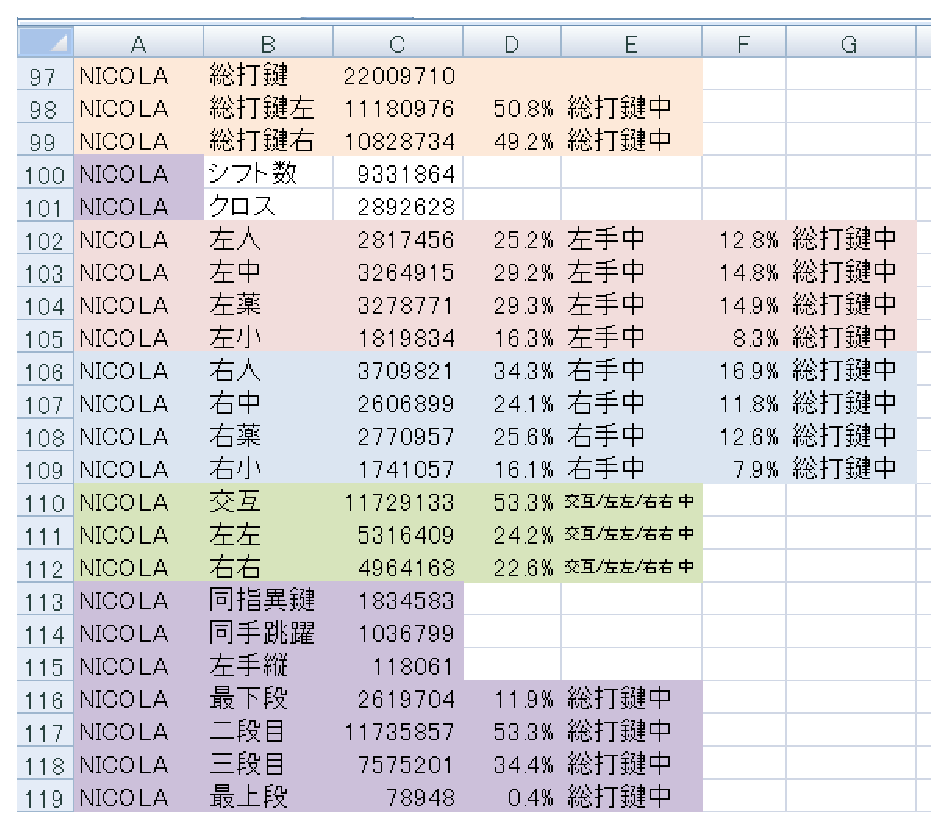
\includegraphics[width=0.85\hsize]{tbl-nicola.eps}
% \end{center}
% \caption{NICOLA配列の解析表}
% \label{tbl:nicola}
%\end{table}

NICOLAではその設計思想通り、左右バランスよく、また、ほどよく交互打鍵がされるように配列されています。
また、ホームポジションの使用率も54\%と、なるべく指から離れないようになっています。
総打鍵中43\%と4割がシフトなのは気になるところですが、ユーザテストによれば気にならないようですので、
よしとしましょう。

なお、シフト数が多いのは「の」「な」「る」などの高頻度の文字がシフトに配列されているためと考えられます。清音キーを非シフトに割り当てねばならなかった宿命でしょう。
参考のため、仮名出現上位20個のうち、裏(シフト側)になってしまった仮名を挙げます\footnote{「約」とつけると見づらいので、省略しました。すべて有効数字は2桁です。}:「の」(5位; 4.0\%)、「に」(9位; 2.8\%)、「な」(11位; 2.5\%)、「る」(15位; 2.2\%)、「っ」(18位; 2.0\%)また、逆に低頻度なのに表に来ざるを得なかった清音の仮名も挙げましょう。「へ」(0.23\%)、「ほ」(0.48\%)、「ふ」(0.48\%)、「ひ」(0.61\%)などなど。

%\subsubsection*{TRON配列}
\subsubsection*{飛鳥配列}

Ray氏によって考案された親指シフト配列である飛鳥配列は、改良に改良を重ねて作られました。その設計思想は
\begin{itemize}
\item 右手をよく使う\footnote{左利きの人用に「レフティ飛鳥」というものも用意されています。}
\item 親指キーを押しっぱなしにした状態での連続入力(裏のキーを連続で入力する)ことを積極的に取り入れている(cf. NICOLAでは一打鍵ごとに一シフト)
\end{itemize}

飛鳥配列はその歴史から大量に版があります%
\footnote{今回用いたのは、飛鳥配列383版のうち、数字の配列が123\ldots となっている「飛鳥配列123-383版」です。}
が、その一例を図\ref{fig:asuka}に示します%
\footnote{図は\url{http://ameblo.jp/asuka-layout/entry-10334710008.html}より。}%
。「がぎぐげご」などの濁音も一つのキーで入力するのが特徴です。

\begin{figure*}[htbp]
 \begin{center}
  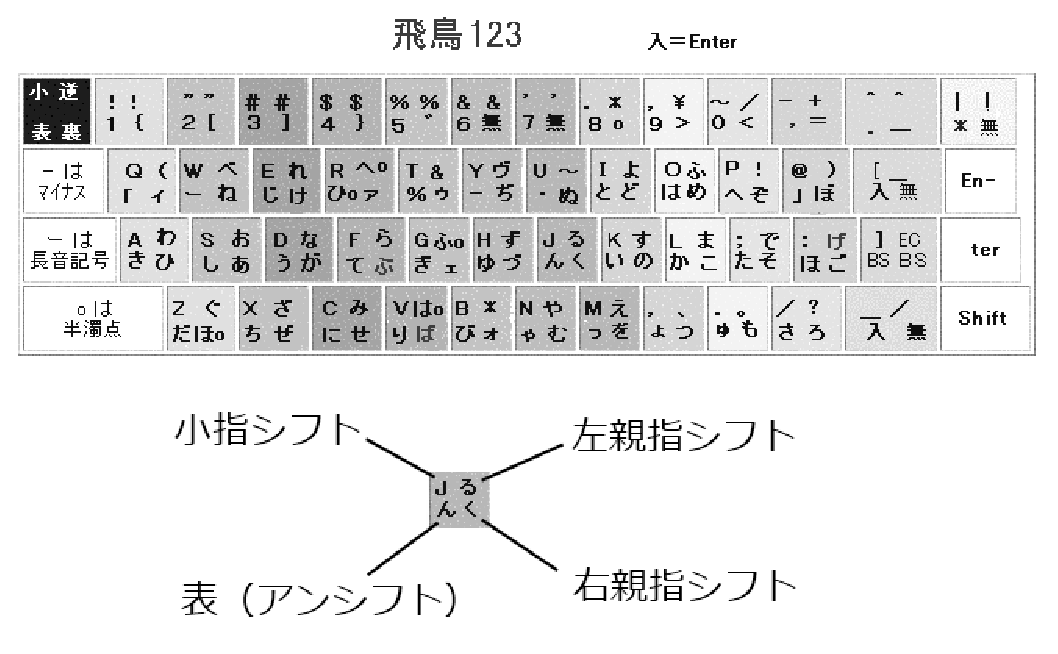
\includegraphics[width=0.8\hsize]{asuka.eps}
 \end{center}
 \caption{飛鳥配列123-383版}
 
 \label{fig:asuka}
\end{figure*}

それではコーパスを使って評価してみます。
%(今回の評価プログラムでは、「シフトを押しっぱなしの連続入力」を定量的に量ることに対応していませんでした。次回以降の課題とします)。

\begin{table*}[htbp]
 \caption{飛鳥配列の解析表}
 \begin{center}
 \begin{tabular}{cccc|ccc}
 \hline
総打鍵 & 総打鍵左 & 総打鍵右 & シフト数 & 交互 & 左左 & 右右 \\
22329794 & 8913749 & 13416045 & 10594571(5240353) & 11489323 & 3169088 & 7671383\\
 & 39.9\% & 60.1\% &  & 65.5\% & 18.1\% & 43.8\%\\
 \hline
 \end{tabular}

  \vspace{1zw} 

 \begin{tabular}{ccccccccccc}
 \hline
& 左小(A) & 左薬(S) & 左中(D) & 左人(FG) & 右人(HJ) & 右中(K) & 右薬(L) & 右小(;)\\
1575536 & 3914260 & 2128521 & 1295432 & 3437742 & 4878650 & 3246516 & 1853137\\
左/右手中 &17.7\% & 43.9\% & 23.9\% & 14.5\% & 25.6\% & 36.4\% & 24.2\% & 13.8\%\\
総打鍵中 & 7.1\% & 17.5\% & 9.5\% & 5.8\% & 15.4\% & 21.8\% & 14.5\% & 8.3\%\\
\hline
 \end{tabular}

  \vspace{1zw} 

 \begin{tabular}{ccc|cccc}
 \hline
 同指異鍵 & 同手跳躍 & 左手縦 & 最下段(ZX..) & ホーム(AS..) & 三段目(QW..) & 最上段(12..)\\
1988288 & 930019 & 20753 & 6033749 & 12828047 & 3389059 & 78939\\
 &  &  & 27.0\% & 57.4\% & 15.2\% & 0.4\%\\
\hline
 \end{tabular}
 \end{center}
 \label{tbl:asuka}
\end{table*}

%\begin{table}[htbp]
% \begin{center}
%  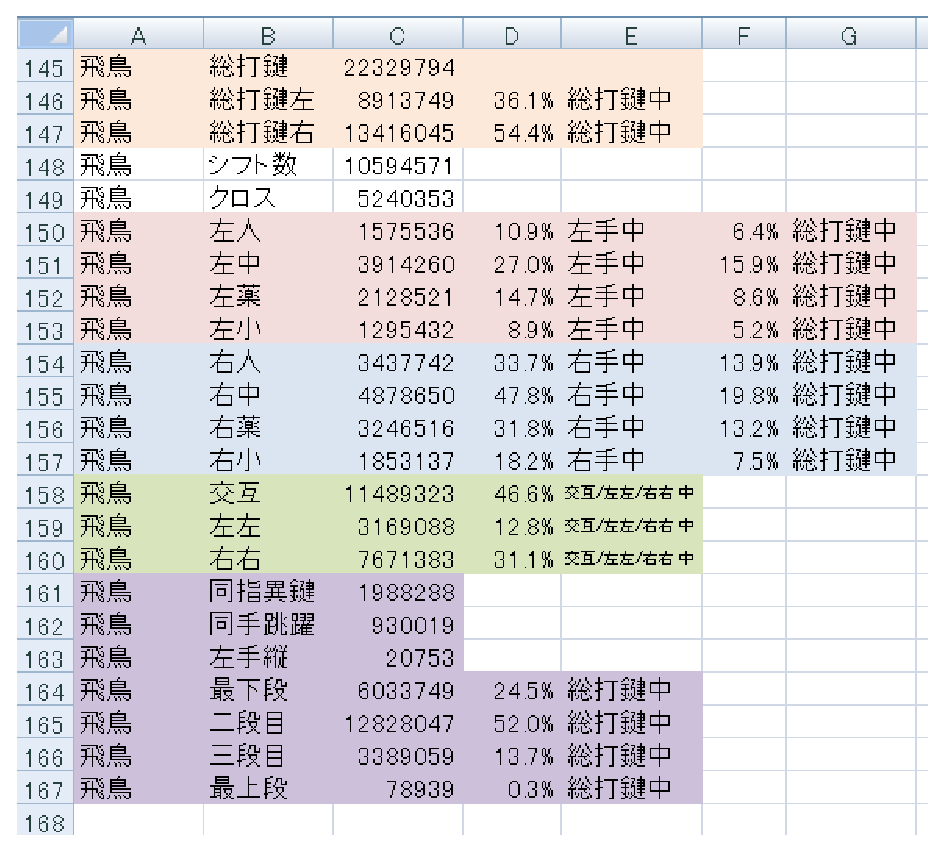
\includegraphics[width=0.85\hsize]{tbl-asuka.eps}
% \end{center}
% \caption{飛鳥配列(383版)の解析表}
% \label{tbl:asuka}
%\end{table}

設計思想通り、右手の使用率が約54\%と高くなっています。また、交互打鍵率が約47\%、続いて右→右の入力が約31\%と、交互打鍵もしつつ、得意な右手を使ってあげるという、バランスのとれた配列になっています。

特筆すべきは左手縦連の少なさです。NICOLAのそれと比べての17\%という少なさです(飛鳥: 20753、NICOLA: 118061)。
飛鳥配列はシフトを押したままの連続入力にあくまでもこだわった結果、アルペジオ運指を多く生み出したのでしょうか(今回使用した解析スクリプトでは、アルペジオ運指は考慮していませんでした。次回以降の課題とします)。

また、最下段の使用もNICOLAに比べて多く、花配列と同様、(パームレストなどを使って)手を浮かせて入力するのに向いていると考えられます。

\subsection*{小梅配列}

小梅配列はNICOLA、TRON配列、飛鳥配列の流れをくむ親指シフト配列で、クロスシフトで濁音を入力する特徴を持っています(図\ref{fig:koume}%
\footnote{図は\url{http://homepage2.nifty.com/61degc/reports/koume/} より。})。

設計思想として、NICOLAと同様にクロスシフトで濁音を入力し、記憶に対する負荷を減らしています。連続シフトではなく、その都度シフトを入力させる点もNICOLAと同様です。
また、交互打鍵率を高くする一方で、多くの人の利き手である右手の使用頻度を高くしています。具体的には、左右の使用頻度を左手:右手=43:57と設定しています(後述するように、これはコーパスでも確認できます)。

\begin{figure*}[htbp]
 \begin{center}
  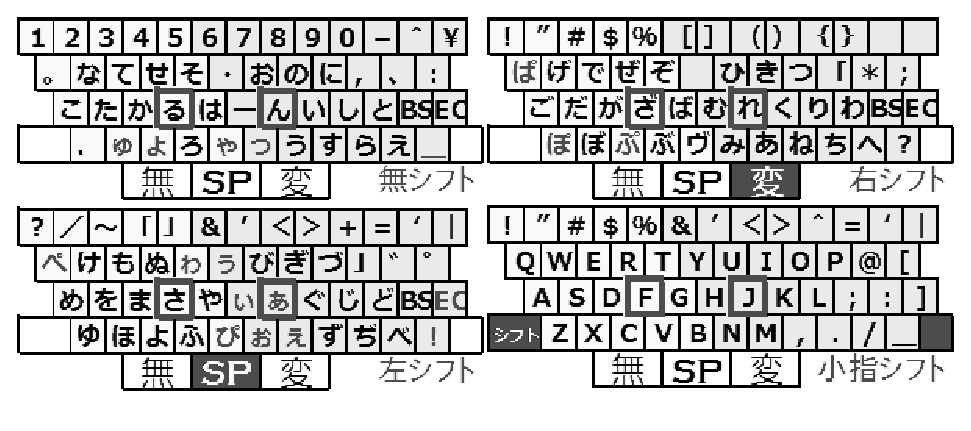
\includegraphics[width=0.8\hsize]{koume.eps}
 \end{center}
 \caption{小梅配列}
 \label{fig:koume}
\end{figure*}

それではコーパスを使って評価してみます。%(今回の評価プログラムでは、「シフトを押しっぱなしの連続入力」を定量的に量ることに対応していませんでした。次回以降の課題とします。)
左手:右手の使用頻度が約44:56と、設計思想通りになっていることがうかがえます。また、交互打鍵率・右手使用率(右→右)もともに高くなっています。

\begin{table*}[htbp]
 \caption{小梅配列の解析表}
 \begin{center}
 \begin{tabular}{cccc|ccc}
 \hline
総打鍵 & 総打鍵左 & 総打鍵右 & シフト数 & 交互 & 左左 & 右右 \\
 22366745 & 9793272 & 12573473 & 8115349(2609182) & 12832519 & 3377012 & 6157214\\
 & 43.8\% & 56.2\% &  & 57.4\% & 15.1\% & 27.5\%\\
 \hline
 \end{tabular}

  \vspace{1zw} 

 \begin{tabular}{ccccccccccc}
 \hline
& 左小(A) & 左薬(S) & 左中(D) & 左人(FG) & 右人(HJ) & 右中(K) & 右薬(L) & 右小(;)\\
& 2620589 & 3462294 & 2461322 & 1249067 & 4025676 & 3719075 & 3191966 & 1636756\\
左/右手中 & 26.8\% & 35.4\% & 25.1\% & 12.8\% & 32.0\% & 29.6\% & 25.4\% & 13.0\%\\
総打鍵中 & 11.7\% & 15.5\% & 11.0\% & 5.6\% & 18.0\% & 16.6\% & 14.3\% & 7.3\%\\
\hline
 \end{tabular}

  \vspace{1zw} 

 \begin{tabular}{ccc|cccc}
 \hline
 同指異鍵 & 同手跳躍 & 左手縦 & 最下段(ZX..) & ホーム(AS..) & 三段目(QW..) & 最上段(12..)\\
1962705 & 1135597 & 18698 & 4734636 & 10838801 & 6627420 & 165888\\
 &  &  & 21.2\% & 48.5\% & 29.6\% & 0.7\%\\
 &  &  & 総打鍵中 & 総打鍵中 & 総打鍵中 & 総打鍵中\\
\hline
 \end{tabular}
 \end{center}
 \label{tbl:roma}
\end{table*}

%\begin{table}[htbp]
% \begin{center}
%  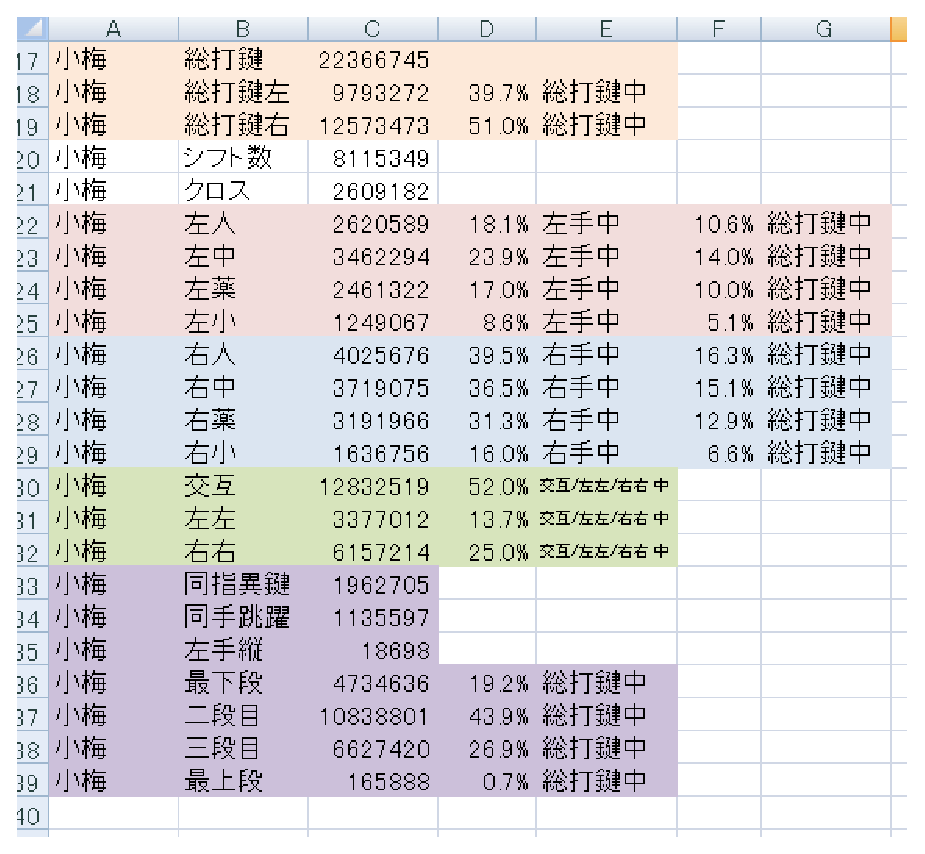
\includegraphics[width=0.85\hsize]{tbl-koume.eps}
% \end{center}
% \caption{小梅配列の解析表}
% \label{tbl:koume}
%\end{table}

\subsection{遺伝的アルゴリズムによる配列決定}

前述の花配列のおさらいをしましょう。花配列では、「よい配列」をまず定義し、ランダムな配置から初めて、組み合わせを少しずつ「よい方向へ」変えていったのでした。
このように、「よさ」({\bf 評価値})を定義して、評価値のできるだけ高い(最大となるのが望ましい)解を求める問題を「探索問題」と言います。
特に、解が配列のような組み合わせの場合、「{\bf 組み合わせ最適化問題}」と呼びます。

一般に、組み合わせ最適化問題は組み合わせの数が膨大になってしまうため、探索が困難です。たとえば、仮名の文字55個と記号8個の計63個を単純に並べる並べ方は$63!$通りです。
これは$10^{87}$よりも$2^{289}$よりも大きい数で、この組み合わせをすべて探索(全解探索、あるいは全探索といいます)するのは現実的ではありません。

そこで、全探索をしないでできるだけよい解を求めるアルゴリズムがいくつも存在します。今から説明するのは、生物の遺伝子を模した「遺伝的アルゴリズム」というものです。
{\bf 遺伝的アルゴリズム}は、解の候補を「遺伝子」という形で表現し、それらを「かけあわせ」(\ruby{{\bf 交叉}}{こうさ})て新しい個体(解)を生成し、
さらに評価値によって「一部のみ生き残らせる」(=自然\ruby{淘汰}{とうた}; {\bf 選択})ことを繰り返すことによって、よりよい解を探索します。
また、交叉の際に解の一部を変化させる(突然{\bf 変異})こともします。
このように、生物の進化を模しているため、進化的アルゴリズムの一種とされます。

しかし、ある仮名配列と仮名配列を単純にかけあわせる(混ぜる)だけでは、同じキーが二カ所出てきたり、存在しないキーが出てきたりと、使いものにならない配列ができてしまいます。
このような配列(遺伝子)を「{\bf 致死遺伝子}」と言います。
致死遺伝子を発生させない交叉をどう実現するか、あるいはそもそも遺伝子をどう表現するかは、とても難しい問題です。

また、評価値の計算も重要です。遺伝的アルゴリズムでは、単一の評価値を用いて生き残る遺伝子を決めていました。
適切な評価基準を用いないと、ふさわしくない遺伝子が生き残ってしまうことになり、やはりよい解は得られません。

このように使いどころが難しい遺伝的アルゴリズムですが、
一般に全探索が困難な問題に対してそれなりに良い解が求められるということで、
一時期、一世を\ruby{風靡}{ふうび}したという過去を持ちます。

\subsubsection*{先行研究(仮名配列以外)}

遺伝的アルゴリズムによるキーボード配列設計では、北インドで話されているヒンディー語の
キーボードの設計 [Deshwal and Kalyanmoy, 2003]や、アルファベットのソフトウェアキーボードの設計 [Raynal and Vigouroux, 2005] などで行われています。

Deshwalらの設計では、二つの遺伝子(配列)$G_1$と$G_2$があったとき、まず$G_1$の半分を残し、
残りの半分のキーを$G_2$のキーの「近く」に並べ替える(=$G_2$のキーを参考にして改良する)
ことで、致死遺伝子を作ることなく交叉を実現しています。
また、評価関数として、交互打鍵率を増やす、同じ指でキーを打たない、などを用いています。

Raynalらは、前提知識編で紹介したフィッツの法則を用いています。ソフトウェアキーボードではマウスやペンを使うので、フィッツの法則がクリティカルに効いてくるのでしょう。

\subsubsection*{幸花配列(旧名:○配列)}

遺伝的アルゴリズムを中指シフト仮名配列の設計に用いたのが、幸花配列(旧名:○配列)です%
\footnote{\url{http://www.geocities.jp/rage2050a/GeneKana/_ReadMe.html}}%
(図\ref{fig:maru})。

\begin{figure*}[htbp]
 \begin{center}
  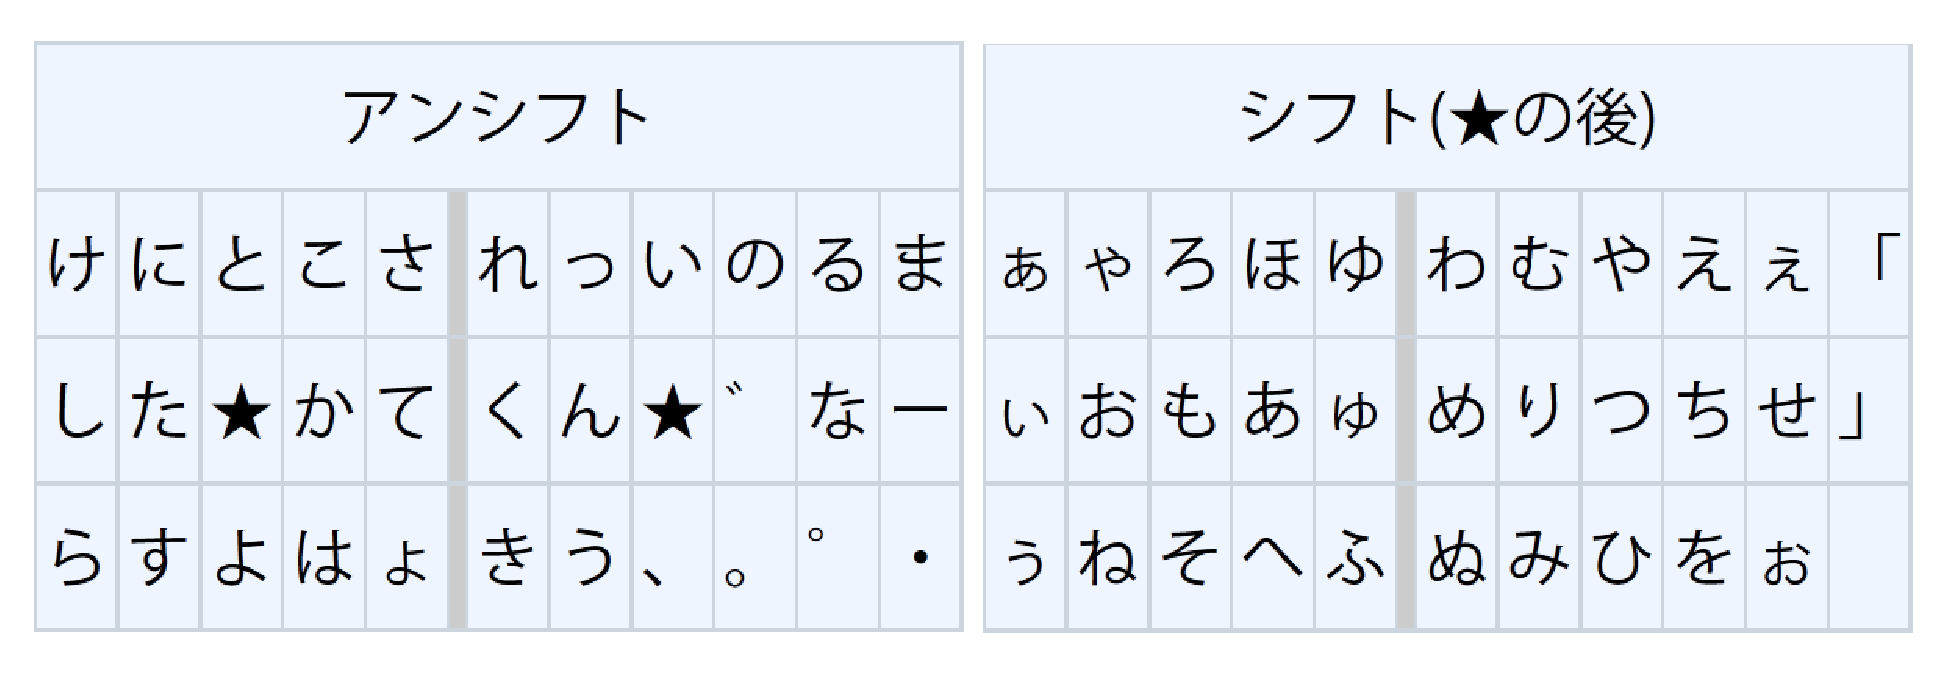
\includegraphics[width=0.8\hsize]{maru.eps}
 \end{center}
 \caption{○配列}
 \label{fig:maru}
\end{figure*}

交叉は、ランダムにキーの位置を選び、ランダムに配列(遺伝子)$G_1$、$G_2$のどちらかを選んでいき、
すべてのキーに仮名を置くまで繰り返す、というものです。
競合が起こる(同じ仮名がすでに置かれている)場合には、
キー配列の左上から順にまだ置かれていないものを選ぶ、という方法で解決しています。
評価には開発者が自身でキーのbigramについて打鍵時間を計測し、その組み合わせを用いました。

それではコーパスを使って評価してみましょう(表\ref{tbl:maru})。

\begin{table*}[htbp]
 \caption{○配列の解析表}
 \begin{center}
 \begin{tabular}{cccc|ccc}
 \hline
総打鍵 & 総打鍵左 & 総打鍵右 & シフト数 & 交互 & 左左 & 右右 \\
29756111 & 14149812 & 15606299 & 5049787 & 19866174 & 4216725 & 5673212\\
 & 47.6\% & 52.4\% &  & 66.8\% & 14.2\% & 19.1\%\\
 \hline
 \end{tabular}

  \vspace{1zw} 

 \begin{tabular}{ccccccccccc}
 \hline
& 左小(A) & 左薬(S) & 左中(D) & 左人(FG) & 右人(HJ) & 右中(K) & 右薬(L) & 右小(;)\\
& 5020769 & 4841928 & 2420872 & 1866243 & 4788744 & 4902439 & 4506402 & 1408714\\
左/右手中 &35.5\% & 34.2\% & 17.1\% & 13.2\% & 30.7\% & 31.4\% & 28.9\% & 9.0\%\\
総打鍵中 & 16.9\% & 16.3\% & 8.1\% & 6.3\% & 16.1\% & 16.5\% & 15.1\% & 4.7\%\\
\hline
 \end{tabular}

  \vspace{1zw} 

 \begin{tabular}{ccc|cccc}
 \hline
 同指異鍵 & 同手跳躍 & 左手縦 & 最下段(ZX..) & ホーム(AS..) & 三段目(QW..) & 最上段(12..)\\
2003058 & 1082831 & 47820 & 5960127 & 16389169 & 7327867 & 78948\\
 &  &  & 20.0\% & 55.1\% & 24.6\% & 0.3\%\\
\hline
 \end{tabular}
 \end{center}
 \label{tbl:maru}
\end{table*}

%\begin{table}[htbp]
% \begin{center}
%  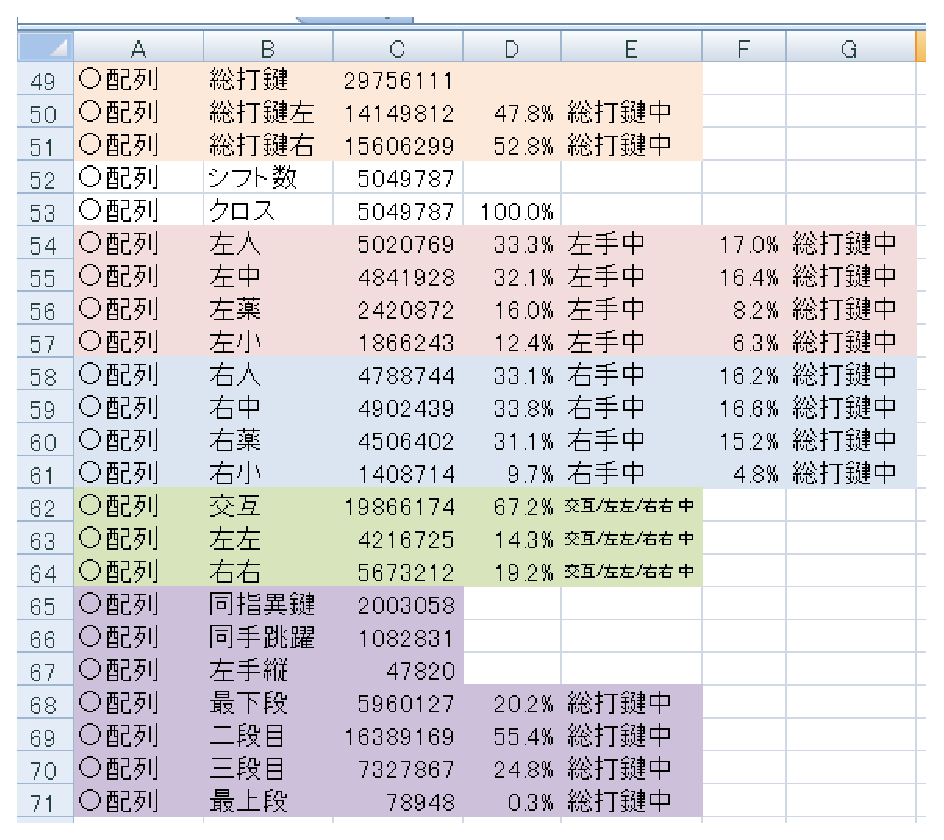
\includegraphics[width=0.85\hsize]{tbl-maru.eps}
% \end{center}
% \caption{○配列の解析表}
% \label{tbl:maru}
%\end{table}

交互打鍵率が約67\%と、花、月配列を若干上回る高さです。
評価値には実測の打鍵時間が用いられているので、交互打鍵の速さを実感できます。

ホームポジションの打鍵率も約55\%と、月、花よりも多くなっています。
左手縦連の少なさ(幸花:47820、花:83290、月:50003)も魅力的です。

\subsection{まとめ}

最後に、今まで出てきた配列をまとめて比較してみましょう(表\ref{tbl:matome}と表\ref{tbl:matome-percent})。
なお、表\ref{tbl:matome-percent}のパーセント表記は、
\begin{itemize}
 \item 総打鍵左・右は総打鍵中の割合
 \item シフト・クロスシフトは総打鍵中の割合
 \item 左\{小薬中人\}・右\{人中薬小\}は総打鍵中に占める割合
 \item (1)交互・(2)左左・(3)右右は、この三つの割合。つまり $ \frac{(1)}{\left\{(1)+(2)+(3)\right\}} $ などの割合。
 \item 最下段~最上段はそれぞれの全打鍵に占める割合(=総打鍵における割合)
\end{itemize}
です。

AZIKのタイプ数の削減率は、中指シフト配列に迫る勢いです。気になるのは左手小指の使用率の高さですが、これはおもに\key{Q}と(前に右手のキーが続くときの-anである)\key{Z}によるものです。実際の運指では、特に「かん」(\key{K}\key{N})などは右だけで打つこともあるため、やや強引な仮定だったかもしれません。

交互打鍵については今回、「中指シフトはすべてクロスシフト」という仮定をおいたため、花/月/幸花(○)配列に有利になっています。
実際の運指によってはアルペジオ運指になることも十分ありえますので、結果を見るときはご注意願います。

交互打鍵を主眼においた新JIS、NICOLA、小梅に比べて、飛鳥配列の交互打鍵率がやや低くなっているのが見てとれます。
飛鳥配列ではその代わり、右右の比率が多くなっており、アルペジオ運指を狙っていることが示唆されます。%
%(ただし、今回の解析プログラムでは、アルペジオについては調べることができませんでした)。

人差し指は二列を担当するため、一般的に使用比率が高くなりがちです。実際、多くの配列で「左人/右人」の値は高くなっています。
一方、飛鳥配列については人差し指の使用率が低くなっていることに注目しましょう。これは飛鳥配列の設計思想の一つ、「人差し指のうち、\key{T}と\key{Y}のある列は遠いので避ける」を反映しているものと言えましょう。

\subsection{あとがき}

今回はQWERTY、および仮名配列に焦点を当てていました。
そのため、Dvorakや、AZIKのDvorak版であるACTに触れることができませんでした。
また、飛鳥配列における連続シフト(アルペジオ運指)についての研究もできませんでした。

先行研究において、「(親指の)シフト動作はタイピングに影響を及ぼさない」とあったとはいえ、
筆者の実感ではシフト動作はわりと指(と頭)に負担がかかっているような印象を受けます。

次回、またこのような文章を書く機会があれば、もっと細かい部分まで凝らした考察を載せたいと考えています。
また、当初の目的であった「打ちやすい」キーボード配列を求めて、配列設計についても文章を\ruby{認}{したた}めたい
です。特に筆者はAZIKに大きな可能性を見いだしているため、今回書いたような知見を活かし、AZIKの最適配置を
計算によって求めたいと思っています。では、またどこかで。

\clearpage

\begin{table*}[htbp]
 \caption{まとめ(値は1000で割ってある)}
 \begin{center}
  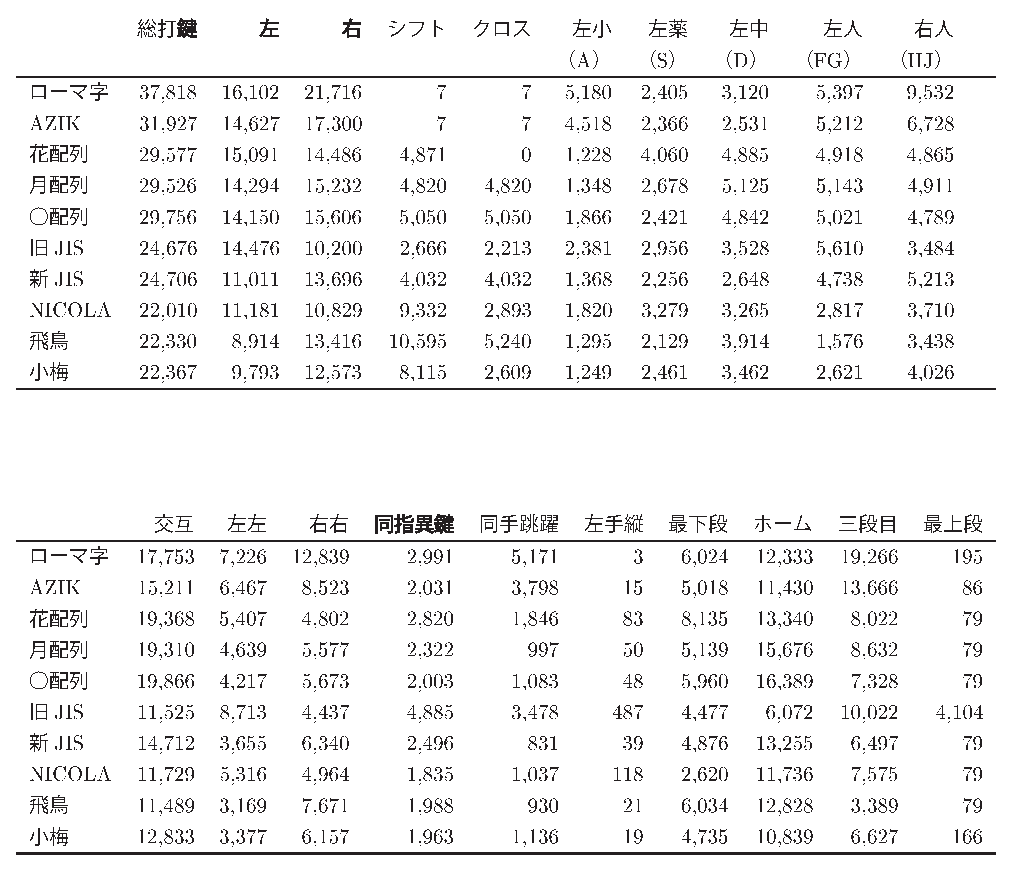
\includegraphics[angle=90, width=0.85\hsize]{matome-table.eps}
 \end{center}
 \label{tbl:matome}
\end{table*}

\clearpage

\begin{table*}[htbp]
 \caption{まとめ(パーセント表記)}
 \begin{center}
  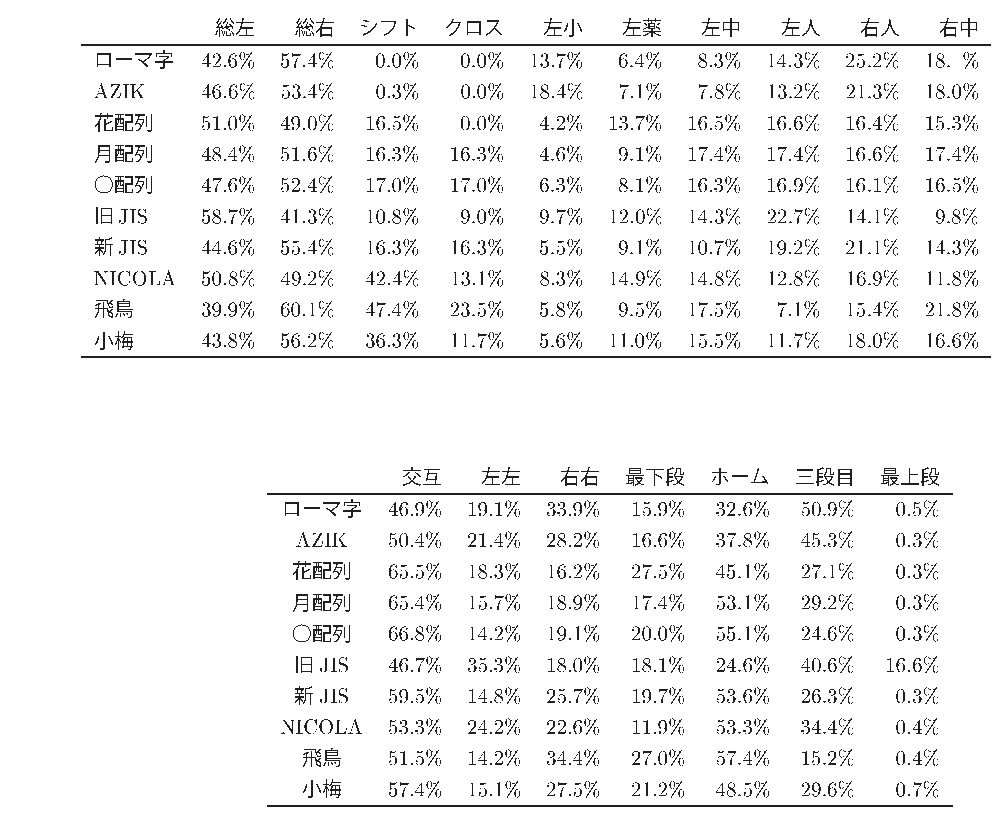
\includegraphics[angle=90, width=0.85\hsize]{matome-table-percent.eps}
 \end{center}
 \label{tbl:matome-percent}
\end{table*}

